%
% Copyright 2018 Joel Feldman, Andrew Rechnitzer and Elyse Yeager.
% This work is licensed under a Creative Commons Attribution-NonCommercial-ShareAlike 4.0 International License.
% https://creativecommons.org/licenses/by-nc-sa/4.0/
%
\questionheader{ex:s1.6}

%%%%%%%%%%%%%%%%%%
\subsection*{\Conceptual}
%%%%%%%%%%%%%%%%%%
\begin{question}
Consider a right circular cone.
\begin{center}
\begin{tikzpicture}
\draw (0,0)node[thin, gray, shape=ellipse, minimum width=3cm, minimum height=1cm, draw, fill=black, fill opacity=0.1] {};
\draw (-1.5,0)--(0,3)--(1.5,0);
\filldraw[draw=blue, left color=blue!50!black, right color=white, opacity=0.3] (-1.5,0)--(0,3)--(1.5,0) arc(0:-180:1.5cm and 0.5cm);

\end{tikzpicture}
\end{center}
What shape are horizontal cross-sections? Are the vertical cross-sections the same?
\end{question}
\begin{hint}
The horizontal cross-sections were discussed in Example~\eref{CLP101}{eg:VOLa} of
the CLP-2 text.
\end{hint}
\begin{answer}
The horizontal cross-sections are circles, but the vertical cross-sections are not.
\end{answer}
\begin{solution}
If we take a horizontal slice of a cone, we get a circle. If we take a vertical cross-section, the base is flat (it's a chord on the circular base of the cone), so we know right away it isn't a circle. Indeed, if we slice down through the very centre, we get a triangle. (Other vertical slices have a curvy top, corresponding to  a class of curves known as hyperbolas.)
\end{solution}

\begin{Mquestion}
Two potters start with a block of clay $h$ units tall, and identical square cookie cutters. They form columns by pushing the square cookie cutter straight down over the clay, so that its cross-section is the same square as the cookie cutter. Potter A pushes their cookie cutter down while their clay block is sitting motionless on a table; Potter B pushes their cookie cutter down while their clay block is rotating on a potter's wheel, so their column looks twisted. Which column has greater volume?

\begin{center}
\hfill
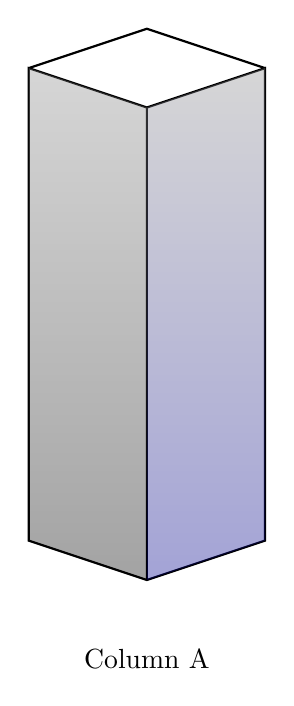
\begin{tikzpicture}
\draw[thick] (-1.5,-3) --(-0,-3.5)--(1.5,-3)--(1.5,3)--(0,2.5)--(-1.5,3)--cycle;
\draw[thick] (-1.5,3)--(0,3.5)--(1.5,3) (0,2.5)--(0,-3.5);
\fill[bottom color=black, top color=white, fill opacity=0.2] (-1.5,3)--(0,2.5)--(0,-3.5)--(-1.5,-3)--cycle;
\fill[bottom color=blue, top color=white, fill opacity=0.2] (1.5,3)--(0,2.5)--(0,-3.5)--(1.5,-3)--cycle;
 \draw (0,-4.5) node {Column A};
\end{tikzpicture}
\hfill
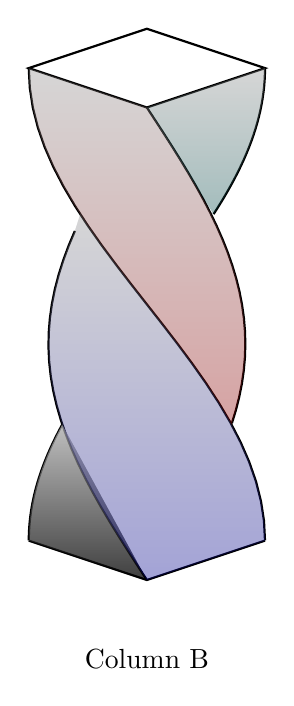
\begin{tikzpicture}
\draw[thick] (-1.5,-3)--(0,-3.5)--(1.5,-3);
\draw[thick] plot[domain=-1.57:1.57]({-1.5*sin(\x r)},1.91*\x);
\draw[thick] (-1.5,3)--(0,2.5)--(1.5,3)--(0,3.5)--cycle;
\draw[thick] plot[domain=-2.1:0, yshift=2.5cm]({-1.25*sin(\x r)},1.91*\x);
\draw[thick] plot[domain=.6:1.57]({1.5*sin(\x r)},1.91*\x);
\draw[thick] plot[domain=-1.57:-.8]({1.5*sin(\x r)},1.91*\x);
\draw[thick] plot[domain=-.75:1.57, yshift=-.5cm]({-1.25*cos(\x r)},-1.91*\x);
\fill[bottom color=black, top color=white, fill opacity=0.5] (0,-3.5)-- plot[domain=-.8:-1.57]({1.5*sin(\x r)},1.91*\x)  plot[domain= .6:1.57, yshift=-.5cm]({-1.25*cos(\x r)},-1.91*\x);
\fill[bottom color=red, top color=white, fill opacity=0.2] (0,2.5) plot[domain=-2.1:0, yshift=2.5cm]({-1.25*sin(\x r)},1.91*\x)--
plot[domain=1.57:-.8]({-1.5*sin(\x r)},1.91*\x)--cycle;
\fill[bottom color=blue, top color=white, fill opacity=0.2] (0,-3.5) --(1.5,-3)
 plot[domain=-1.57:.6]({-1.5*sin(\x r)},1.91*\x)--
plot[domain=-.75:1.57, yshift=-.5cm]({-1.25*cos(\x r)},-1.91*\x);
\fill[bottom color=green!50!blue, top color=white, fill opacity=0.2] (0,2.5) --(1.5,3)
 plot[domain=.6:1.57]({1.5*sin(\x r)},1.91*\x)--(0,2.5)--
 cycle;
 \draw (0,-4.5) node {Column B};
\end{tikzpicture}
\hfill~
\end{center}
\end{Mquestion}
\begin{hint}
What are the dimensions of the cross-sections?
\end{hint}
\begin{answer}
The columns have the same volume.
\end{answer}
\begin{solution}
The columns have the same volume. We can see this by chopping up the columns into horizontal cross-sections. Each cross-section has the same area as the cookie cutter, $A$, and height $\dee{y}$. Then in both cases, the volume of the column is
\[\int_{0}^h A~\dee{y}  = hA \mbox{ cubic units}\]
\end{solution}

%%%%%%%%%%%%%%%%%%
\begin{question}
Let $R$ be the region bounded above by the graph of $y=f(x)$ shown below and bounded below by the $x$-axis, from $x=0$ to $x=6$. Sketch the washers that are formed by rotating $R$ about the $y$-axis.
In your sketch, label all the radii in terms of $y$, and label the thickness.
\begin{center}
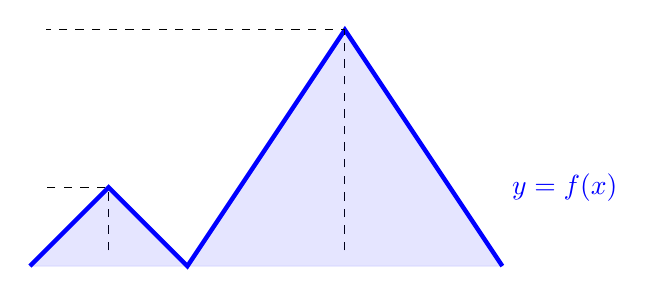
\begin{tikzpicture}
\YEaaxis{1}{7}{1}{4}
\draw[ultra thick, blue] (0,0)--(1,1)--(2,0)--(4,3)--(6,0);
\draw[blue](6,1) node  [right]{$y=f(x)$};
\foreach \x in {2,1,4,6}{\YExcoord{\x}{\x}}
\foreach \x in {1,3}{\YEycoord{\x}{\x}}
\draw[dashed] (1,.2)|-(.2,1) (4,.2)|-(.2,3);
\filldraw[blue, opacity=0.1] (0,0)--(1,1)--(2,0)--(4,3)--(6,0)--cycle;
\end{tikzpicture}
\end{center}

\end{question}
\begin{hint}
There are two different kinds of washers.
\end{hint}
\begin{answer}

\begin{description}
\item[Washers when $\mathbf{1<y \le 6}$:]
If $y>1$, then our washer has inner radius $2+\frac{2}{3}y$, outer radius $6-\frac{2}{3}y$, and height $\dee{y}$.
\begin{center}
\begin{tikzpicture}

\draw node[shape=ellipse, minimum width=6cm, minimum height=3cm, fill=red, fill opacity=0.1]{};
\draw node[shape=ellipse, minimum width=3cm, minimum height=1cm, fill=white]{};


\draw node[shape=ellipse, minimum width=3cm, minimum height=1cm, draw]{};
\draw node[shape=ellipse, minimum width=6cm, minimum height=3cm, draw]{};
\draw (-3,0)--(-3,-.2) arc(180:360:3cm and 1.5cm)--(3,0);
\draw (0,-.15)+(174:1.5cm and .5cm)arc(174:6:1.5cm and .5cm);
\draw (3.5,-.2)-|(3.75,0)--(3.5,0);
\draw[dashed] (0,-3)--(0,-1.7) (0,-.5)--(0,4) node[above]{$y$};
\draw node[vertex]{};
\draw (4,-0.1) node[right]{thickness: $\dee{y}$};
\draw[decorate, decoration={brace, amplitude=10pt}] (0,-2)--(-3,-2) node[midway, yshift=-.75cm]{$R = 6-\frac{2}{3}y$};
\draw[dashed] (-3,0)--(-3,-2);
\draw[decorate, decoration={brace, amplitude=10pt}] (0,2)--(1.5,2) node[midway, yshift=.75cm, xshift=5mm]{$r = 2+\frac{2}{3}y$};
\draw[dashed] (1.5,2)--(1.5,0);
\end{tikzpicture}
\end{center}

\item[Washers when $\mathbf{0\le y <1}$:]
When $0 \le y < 1$, we have a ``double washer," two concentric rings. The inner washer has inner radius $r_1=y$ and outer radius $R_1=2-y$. The outer washer has inner radius $r_2=2+\frac{2}{3}y$ and outer radius $R_2=6-\frac{2}{3}y$. The thickness of the washers is $\dee{y}$.

\begin{center}
\begin{tikzpicture}
\draw[red] node[shape=ellipse, minimum width=15cm, minimum height=9cm, fill=red, fill opacity=0.1]{};
\draw[red] node[shape=ellipse, minimum width=9cm, minimum height=5cm, fill=white]{};

\draw[blue] node[shape=ellipse, minimum width=6cm, minimum height=3cm, fill=blue, fill opacity=0.1]{};
\draw[blue] node[shape=ellipse, minimum width=3cm, minimum height=1cm, fill=white]{};


\draw[blue] node[shape=ellipse, minimum width=3cm, minimum height=1cm, draw]{};
\draw[blue] node[shape=ellipse, minimum width=6cm, minimum height=3cm, draw]{};
\draw[red] node[shape=ellipse, minimum width=9cm, minimum height=5cm, draw]{};
\draw[red] node[shape=ellipse, minimum width=15cm, minimum height=9cm, draw]{};
\draw[blue] (-3,0)--(-3,-.2) arc(180:360:3cm and 1.5cm)--(3,0);
\draw[blue] (0,-.15)+(174:1.5cm and .5cm)arc(174:6:1.5cm and .5cm);
\draw[red] (0,-.15)+(174:4.5cm and 2.5cm)arc(174:6:4.5cm and 2.5cm);
\draw[red] (-7.5,0)--(-7.5,-.2) arc(180:360:7.5cm and 4.5cm)--(7.5,0);
\draw (3.5,-.2)-|(3.75,0)--(3.5,0);
\draw[dashed] (0,-5)--(0,-4.7)  (0,-2.5)--(0,-1.7) (0,-.5)--(0,6) node[above]{$y$};
\draw node[vertex]{};
\draw (4,-0.1) node[right]{thickness: $\dee{y}$};
\draw[blue, decorate, decoration={brace, amplitude=10pt}] (3,-1.75)--(0,-1.75) node[midway, yshift=-1.cm]{$R_1 = 2-y$};
\draw[dashed, blue] (3,0)--(3,-1.75);


\draw[red, decorate, decoration={brace, amplitude=10pt}] (0,-5)--(-7.5,-5) node[midway, yshift=-.75cm]{$R_2 = 6-\frac{2}{3}y$};
\draw[dashed, red] (-7.5,0)--(-7.5,-5);
\draw[blue, decorate, decoration={brace, amplitude=10pt}] (0,1)--(1.5,1) node[midway, yshift=.75cm, xshift=5mm]{$r_1 = y$};
\draw[dashed, blue] (1.5,1)--(1.5,0);
\draw[red, decorate, decoration={brace, amplitude=10pt}] (-4.5,3)--(0,3) node[midway, yshift=.75cm, xshift=5mm]{$r_2 = 2+\frac{2}{3}y$};
\draw[dashed, red] (-4.5,3)--(-4.5,0);

\end{tikzpicture}
\end{center}

\end{description}
\end{answer}
\begin{solution}
Notice $f(x)$ is a piecewise linear function, so we can find explicit equations for each of its pieces from the graph. The radii will be determined by the $x$-values, so below we give the $x$-values as functions of $y$.

\begin{center}
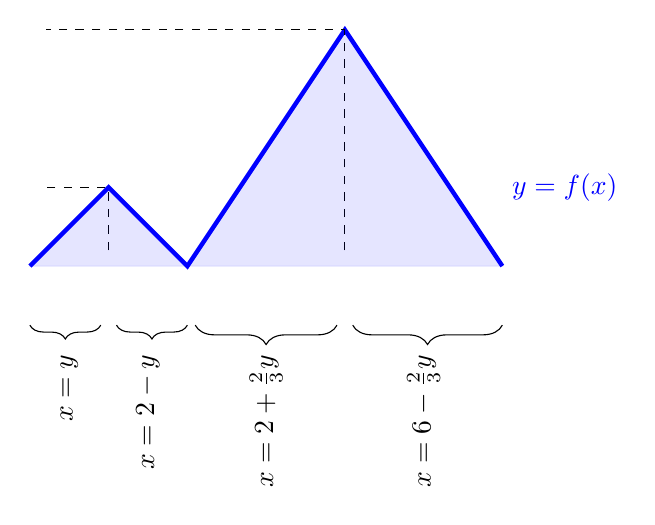
\begin{tikzpicture}
\YEaaxis{1}{7}{1}{4}
\draw[ultra thick, blue] (0,0)--(1,1)--(2,0)--(4,3)--(6,0);
\draw[blue](6,1) node  [right]{$y=f(x)$};
\foreach \x in {2,1,4,6}{\YExcoord{\x}{\x}}
\foreach \x in {1,3}{\YEycoord{\x}{\x}}
\draw[dashed] (1,.2)|-(.2,1) (4,.2)|-(.2,3);
\filldraw[blue, opacity=0.1] (0,0)--(1,1)--(2,0)--(4,3)--(6,0)--cycle;

\draw[decorate, decoration={brace, amplitude=5pt}] (.9,-.75)--(0,-.75);
\draw (.5,-1) node[rotate=90, left]{$x=y$};
\draw[decorate, decoration={brace, amplitude=5pt}] (2,-.75)--(1.1,-.75);
\draw (1.5,-1) node[rotate=90, left]{$x=2-y$};
\draw[decorate, decoration={brace, amplitude=7pt}] (3.9,-.75)--(2.1,-.75);
\draw (3,-1) node[rotate=90, left]{$x=2+\frac{2}{3}y$};
\draw[decorate, decoration={brace, amplitude=7pt}] (6,-.75)--(4.1,-.75);
\draw (5,-1) node[rotate=90, left]{$x=6-\frac{2}{3}y$};
\end{tikzpicture}
\end{center}



If we imagine rotating the region from the picture about the $y$-axis, there will be two kinds of washers formed: when $y<1$, we have a ``double washer," two concentric rings. When $y>1$, we have a single ring.

\begin{description}
\item[Washers when $\mathbf{1<y \le 6}$:]
If $y>1$, then our washer has inner radius $2+\frac{2}{3}y$, outer radius $6-\frac{2}{3}y$, and height $\dee{y}$.
\begin{center}
\begin{tikzpicture}

\draw node[shape=ellipse, minimum width=6cm, minimum height=3cm, fill=red, fill opacity=0.1]{};
\draw node[shape=ellipse, minimum width=3cm, minimum height=1cm, fill=white]{};


\draw node[shape=ellipse, minimum width=3cm, minimum height=1cm, draw]{};
\draw node[shape=ellipse, minimum width=6cm, minimum height=3cm, draw]{};
\draw (-3,0)--(-3,-.2) arc(180:360:3cm and 1.5cm)--(3,0);
\draw (0,-.15)+(174:1.5cm and .5cm)arc(174:6:1.5cm and .5cm);
\draw (3.5,-.2)-|(3.75,0)--(3.5,0);
\draw[dashed] (0,-3)--(0,-1.7) (0,-.5)--(0,4) node[above]{$y$};
\draw node[vertex]{};
\draw (4,-0.1) node[right]{thickness: $\dee{y}$};
\draw[decorate, decoration={brace, amplitude=10pt}] (0,-2)--(-3,-2) node[midway, yshift=-.75cm]{$R = 6-\frac{2}{3}y$};
\draw[dashed] (-3,0)--(-3,-2);
\draw[decorate, decoration={brace, amplitude=10pt}] (0,2)--(1.5,2) node[midway, yshift=.75cm, xshift=5mm]{$r = 2+\frac{2}{3}y$};
\draw[dashed] (1.5,2)--(1.5,0);
\end{tikzpicture}
\end{center}

\item[Washers when $\mathbf{0\le y <1}$:]
When $0 \le y < 1$, we have a ``double washer," two concentric rings corresponding to the two ``humps" in the function.  The inner washer has inner radius $r_1=y$ and outer radius $R_1=2-y$. The outer washer has inner radius $r_2=2+\frac{2}{3}y$ and outer radius $R_2=6-\frac{2}{3}y$. The thickness of the washers is $\dee{y}$.

\begin{center}
\begin{tikzpicture}
\draw[red] node[shape=ellipse, minimum width=15cm, minimum height=9cm, fill=red, fill opacity=0.1]{};
\draw[red] node[shape=ellipse, minimum width=9cm, minimum height=5cm, fill=white]{};

\draw[blue] node[shape=ellipse, minimum width=6cm, minimum height=3cm, fill=blue, fill opacity=0.1]{};
\draw[blue] node[shape=ellipse, minimum width=3cm, minimum height=1cm, fill=white]{};


\draw[blue] node[shape=ellipse, minimum width=3cm, minimum height=1cm, draw]{};
\draw[blue] node[shape=ellipse, minimum width=6cm, minimum height=3cm, draw]{};
\draw[red] node[shape=ellipse, minimum width=9cm, minimum height=5cm, draw]{};
\draw[red] node[shape=ellipse, minimum width=15cm, minimum height=9cm, draw]{};
\draw[blue] (-3,0)--(-3,-.2) arc(180:360:3cm and 1.5cm)--(3,0);
\draw[blue] (0,-.15)+(174:1.5cm and .5cm)arc(174:6:1.5cm and .5cm);
\draw[red] (0,-.15)+(174:4.5cm and 2.5cm)arc(174:6:4.5cm and 2.5cm);
\draw[red] (-7.5,0)--(-7.5,-.2) arc(180:360:7.5cm and 4.5cm)--(7.5,0);
\draw (3.5,-.2)-|(3.75,0)--(3.5,0);
\draw[dashed] (0,-5)--(0,-4.7)  (0,-2.5)--(0,-1.7) (0,-.5)--(0,6) node[above]{$y$};
\draw node[vertex]{};
\draw (4,-0.1) node[right]{thickness: $\dee{y}$};
\draw[blue, decorate, decoration={brace, amplitude=10pt}] (3,-1.75)--(0,-1.75) node[midway, yshift=-1.cm]{$R_1 = 2-y$};
\draw[dashed, blue] (3,0)--(3,-1.75);


\draw[red, decorate, decoration={brace, amplitude=10pt}] (0,-5)--(-7.5,-5) node[midway, yshift=-.75cm]{$R_2 = 6-\frac{2}{3}y$};
\draw[dashed, red] (-7.5,0)--(-7.5,-5);
\draw[blue, decorate, decoration={brace, amplitude=10pt}] (0,1)--(1.5,1) node[midway, yshift=.75cm, xshift=5mm]{$r_1 = y$};
\draw[dashed, blue] (1.5,1)--(1.5,0);
\draw[red, decorate, decoration={brace, amplitude=10pt}] (-4.5,3)--(0,3) node[midway, yshift=.75cm, xshift=5mm]{$r_2 = 2+\frac{2}{3}y$};
\draw[dashed, red] (-4.5,3)--(-4.5,0);

\end{tikzpicture}
\end{center}

\end{description}
\end{solution}
%%%%%%%%%%%%%%%%%%

%%%%%%%%%%%%%%%%%%%%%%%%%%%%%%%%%%%%%

\begin{question}[2000D]  %% 1
Write down definite integrals that represent the following quantities.
\emph{Do not evaluate the integrals explicitly.}
\begin{enumerate}[(a)]
\item
The volume of the solid obtained by rotating  around the $x$--axis the
region between the $x$--axis and $y=\sqrt{x}\, e^{x^2}$ for $0\le x\le 3$.
\item
The volume of the solid obtained by revolving the
region bounded by the curves $y=x^2$ and $y=x+2$ about the line $x=3$.
\end{enumerate}
\end{question}

\begin{hint}
Draw sketches.
The mechanically easiest way to answer part (b) uses the method of cylindrical
shells, which is in the optional section \eref{CLP101}{sec int volumes}
                of the CLP-2 text.  The method of washers also works, but requires  you to have more patience and also
to have a good idea what the specified region looks like.  Look at your sketch
very careful when identifying the ends of your horizontal strips.
\end{hint}

\begin{answer} (a)
$\pi\displaystyle\int_{0}^{3} xe^{2x^2}\ \dee{x}$

\noindent (b)
$\displaystyle\int _0^1  \pi\big[\big(3+\sqrt{y}\big)^2-\big(3-\sqrt{y}\big)^2\big]\dee{y}
+\displaystyle\int _ 1^4  \pi\big[\big(5-y\big)^2-\big(3-\sqrt{y}\big)^2\big]\dee{y}$

\end{answer}

\begin{solution} (a)
When the strip shown in the figure
\begin{center}
       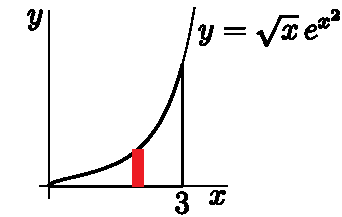
\includegraphics{OE00D_3b}
\end{center}

\noindent  is rotated about the $x$--axis, it
forms a thin disk of radius $\sqrt{x}e^{x^2}$  and thickness $\dee{x}$
and hence of cross sectional area $\pi xe^{2x^2}$ and volume $\pi xe^{2x^2}\,\dee{x}$
So the volume of the solid is
\begin{align*}
\pi\int_{0}^{3} xe^{2x^2}\ \dee{x}
\end{align*}


\noindent (b)
The curves intersect at $(-1,1)$ and $(2,4)$.

\begin{center}
       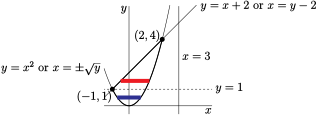
\includegraphics[scale=1.2]{OE00D_3e}
\end{center}

\noindent
We'll use horizontal washers as in Example  \eref{CLP101}{eg rot yaxis}
of the %\href{http://www.math.ubc.ca/%7Efeldman/m101/clp/clp_notes_101.pdf}{CLP 101 notes}.
CLP-2 text.
 \begin{itemize}
\item We use thin horizontal  strips of width $\dee{y}$ as in the figure  above.

\item When we rotate about the line $x=3$, each strip
sweeps out a thin washer
\begin{itemize}
\item
whose inner radius is $r_{in}=3-\sqrt{y}$, and
\item
whose outer radius is $r_{out}=3-(y-2)=5-y$ when $y\ge 1$
(see the red strip in the figure on the right above),  and
whose outer radius is $r_{out}= 3-(-\sqrt{y})=3+\sqrt{y}$ when $y\le 1$
(see the blue strip in the figure on the right above) and
\item
whose thickness is $\dee{y}$ and hence
\item
whose volume is
$\pi(r_{out}^2 - r_{in}^2)\dee{y}
       = \pi\big[\big(5-y\big)^2-\big(3-\sqrt{y}\big)^2\big]\dee{y}$
when $y\ge 1$ and  whose volume is
$\pi(r_{out}^2 - r_{in}^2)\dee{y}
    =\pi\big[\big(3+\sqrt{y}\big)^2-\big(3-\sqrt{y}\big)^2\big]\dee{y}$
when $y\le 1$ and

\end{itemize}
\item As our bottommost strip is at $y=0$ and our topmost
strip is at $y=4$, the total volume is
\begin{align*}
\int _0^1  \pi\big[\big(3+\sqrt{y}\big)^2-\big(3-\sqrt{y}\big)^2\big]\dee{y}
+\int _ 1^4  \pi\big[\big(5-y\big)^2-\big(3-\sqrt{y}\big)^2\big]\dee{y}
\end{align*}
\end{itemize}

\end{solution}
%%%%%%%%%%%%%%%%%%%%%%%%%%%%%%%%%%%%%%%%

\begin{Mquestion}[2001A,M121 2001A]  %% 2
Write down definite integrals that represent the following quantities.
\emph{Do not evaluate the integrals explicitly.}
\begin{enumerate}[(a)]
\item
The volume of the solid obtained by rotating the finite plane
region bounded by the curves $y=1-x^2$ and $y=4-4x^2$ about the line $y=-1$.
\item
The volume of the solid obtained by rotating the finite plane
region bounded by the curve $y=x^2-1$ and the line $y=0$ about the line $x=5$.
\end{enumerate}
\end{Mquestion}

\begin{hint}
Draw sketchs.
\end{hint}

\begin{answer} (a)
$\displaystyle\int_{-1}^{1}\pi\big[{(5-4x^2)}^2-{(2-x^2)}^2\big]\,\dee{x}$
\qquad (b)
$\displaystyle\int _{-1}^0   \pi\big[\big(5+\sqrt{y+1}\big)^2-\big(5-\sqrt{y+1}\big)^2\big]\,\dee{y}$

\end{answer}

\begin{solution} (a)
The curves intersect at $(1,0)$ and $(-1,0)$. When the strip shown in the
figure
\begin{center}
       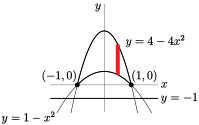
\includegraphics{OE01A_2b}
\end{center}

\noindent
is rotated about the line $y=-1$, it forms a thin washer with:
\begin{itemize}
\item
inner radius  $(1-x^2)-(-1)=2-x^2$,
\item
outer radius $(4-4x^2)-(-1)=5-4x^2$  and
\item thickness $\dee{x}$\ ; so, it has
\item
cross sectional area $\pi\big[{(5-4x^2)}^2-{(2-x^2)}^2\big]$ and
\item
volume $\pi\big[{(5-4x^2)}^2-({2-x^2)}^2\big]\,\dee{x}$.
\end{itemize}

\noindent So the volume of the solid is
\begin{align*}
\int_{-1}^{1}\pi\big[{(5-4x^2)}^2-{(2-x^2)}^2\big]\,\dee{x}
\end{align*}


\noindent (b)
The curve $y=x^2-1$ intersects $y=0$ at $(1,0)$ and $(-1,0)$.

\begin{center}
       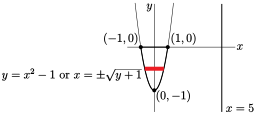
\includegraphics[scale=1.2]{OE01A_2c}
\end{center}

\noindent
We'll use horizontal washers.
 \begin{itemize}
\item We use thin horizontal  strips of height $\dee{y}$ as in the figure  above.

\item
When we rotate about the line $x=5$, each strip sweeps out a thin washer
\begin{itemize}
\item
whose inner radius is $r_{in}=5-\sqrt{y+1}$, and
\item
whose outer radius is $r_{out}= 5-(-\sqrt{y+1})=5+\sqrt{y+1}$ and
\item
whose thickness is $\dee{y}$ and hence
\item
whose volume is
$\pi(r_{out}^2 - r_{in}^2)\,\dee{y}
       = \pi\big[\big(5+\sqrt{y+1}\big)^2-\big(5-\sqrt{y+1}\big)^2\big]\,\dee{y}$

\end{itemize}
\item As our topmost strip is at $y=0$ and our bottommost
strip is at $y=-1$ (when $x=0$), the total volume is
\begin{align*}
\int _{-1}^0   \pi\left[\big(5+\sqrt{y+1}\big)^2-\big(5-\sqrt{y+1}\big)^2\right]\,\dee{y}
\end{align*}
\end{itemize}

\end{solution}
%%%%%%%%%%%%%%%%%%%%%%%%%%%%%%%%%%%%%%%%


\begin{question}[2001D] %% 3
Write down a definite integral that represents the volume of the solid
obtained by rotating  around the line $y=-1$ the region between the
curves $y=x^2$ and $y=8-x^2$.
\emph{Do not evaluate the integrals explicitly.}
\end{question}

\begin{hint}
Draw a sketch.
\end{hint}

\begin{answer}
$\pi\displaystyle\int_{-2}^{2}\big[{(9-x^2)}^2-{(x^2+1)}^2\big]\ \dee{x}$
\end{answer}

\begin{solution}
The curves intersect at $(-2,4)$ and $(2,4)$. When the strip
shown in the figure
\begin{center}
       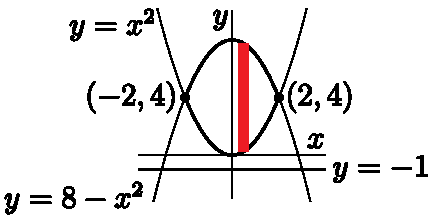
\includegraphics{OE01D_3b}
\end{center}

\noindent
is rotated about the line $y=-1$, it forms
a thin washer (punctured disc) of
\begin{itemize}
\item
inner radius $x^2+1$,
\item
outer radius $9-x^2$  and
\item thickness $\dee{x}$ and hence of
\item
cross sectional area $\pi\big[{(9-x^2)}^2-{(x^2+1)}^2\big]$ and
\item
volume $\pi\big[{(9-x^2)}^2-{(x^2+1)}^2\big]\,\dee{x}$.
\end{itemize}

\noindent So the volume of the solid is
\begin{align*}
\pi\int_{-2}^{2}\big[{(9-x^2)}^2-{(x^2+1)}^2\big]\ \dee{x}
\end{align*}
\end{solution}
%%%%%%%%%%%%%%%%%%%%%%%%%%%%%%%%%%%%%%%%

%%%-------all three parts were asked before
%\begin{question}[M121 2001A] %% 4
%Write definite integrals that represent the following quantities.
%\emph{Do not evaluate the integrals.}
%\begin{enumerate}[(a)]
%\item
%The area of the finite plane region bounded by $y^2=4ax$ and
%$x^2=4ay$, where $a>0$ is a constant.
%\item
%The volume of the solid obtained by rotating the finite plane
%region bounded by the curves $y=1-x^2$ and $y=4-4x^2$ about the line $y=-1$.
%\item
% The volume of the solid obtained by rotating the finite plane
%region bounded by the curve $y=x^2-1$ and the line $y=0$ about the line $x=5$.
%\end{enumerate}
%\end{question}

%\begin{hint}
%(a) Draw a sketch.
%\qquad
%(b) Draw a sketch.
%\qquad
%(c) Draw a sketch.
%\qquad
%See a pattern?
%\end{hint}

%\begin{answer}
%(a) $\displaystyle\int_0^{4a}\left[\sqrt{4ax}-\frac{x^2}{4a}\right]\ \dee{x}$
%\qquad
%(b) $\displaystyle\int_{-1}^{1}\pi\big[{(5-4x^2)}^2-{(2-x^2)}^2\big]\ \dee{x}$

%\noindent
%(c) $\displaystyle\int_{-1}^0\pi\big[{(5+\sqrt{y+1})}^2-{(5-\sqrt{y+1})}^2\big]\ \dee{y}
%=\displaystyle\int_{-1}^020\pi\sqrt{y+1}\,\dee{y}$
%\end{answer}

%\begin{solution} (a) (This was also calculated in Section 1.5, Question~\ref{1.5_4ax4ay}.)
%The curves intersect at points $(x,y)$ which satisfy both
%$y^2=4ax$ and $x^2=4ay$. Substituting $y=\frac{x^2}{4a}$ (from
%the second equation) into the first equation gives
%\begin{equation*}
%\frac{x^4}{4^2a^2}=4ax
%\iff x^4=4^3a^3x
%\iff x(x^3-4^3a^3)=0
%\end{equation*}
%This has two solutions: $x=0$ and $x=4a$. The corresponding values
%of $y$ are $y=0$ and $y=4a$. So the curves intesect at $(0,0)$ and $(4a,4a)$.
%The strip shown in the figure

%\begin{center}
%       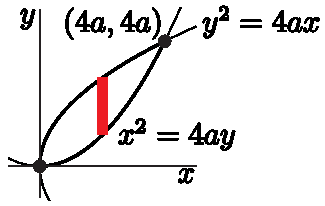
\includegraphics{E121_01A_1a}
%\end{center}

%\noindent runs from $y=B(x) = \frac{x^2}{4a}$ (gotten by solving
%$x^2=4ay$ for $y$) to $y=T(x)= \sqrt{4ax}$
%(gotten by solving $y^2=4ax$ for $y$) and hence has height
%$T(x)-B(x) = \sqrt{4ax}-\frac{x^2}{4a}$ and width $\dee{x}$.
%So the desired
%\begin{equation*}
%{\rm Area} = \int_0^{4a}\Big[\sqrt{4ax}-\frac{x^2}{4a}\Big]\ \dee{x}
%\end{equation*}

%\noindent (b)
%The curves intersect at points $(x,y)$ which satisfy both
%$y=1-x^2$ and $y=4(1-x^2)$. That is, where
%\begin{equation*}
%1-x^2=4(1-x^2)
%\iff 3(1-x^2)=0\iff x=\pm 1
%\end{equation*}
%Thus the curves intersect at $(1,0)$ and $(-1,0)$. When the strip
%shown in the figure

%\begin{center}
%       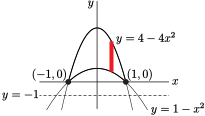
\includegraphics{E121_01A_1b}
%\end{center}

%\noindent
%is rotated about the line $y=-1$, it forms
%a thin washer (punctured disc) of
%\begin{itemize}
%\item
%inner radius $(1-x^2)-(-1)=2-x^2$,
%\item
%outer radius $(4-4x^2)-(-1)=5-4x^2$  and
%\item thickness $\dee{x}$ and hence of
%\item
%cross sectional area $\pi\big[{(5-4x^2)}^2-{(2-x^2)}^2\big]$ and
%\item
%volume $\pi\big[{5-4x^2)}^2-{(2-x^2)}^2\big]\,\dee{x}$.
%\end{itemize}

%\noindent So the volume of the solid is
%\begin{align*}
%\int_{-1}^{1}\pi\big[{(5-4x^2)}^2-{(2-x^2)}^2\big]\ \dee{x}
%\end{align*}


%\noindent (c)
%Note that solving $y=x^2-1$ for $x$ gives $x=\pm\sqrt{y+1}$.
%When the strip shown in the figure

%\begin{center}
%       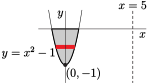
\includegraphics{E121_01A_1c}
%\end{center}

%\noindent
%is rotated about the line $x=5$, it forms
%a thin washer (punctured disc) of
%\begin{itemize}
%\item
%inner radius $5-\sqrt{y+1}$,
%\item
%outer radius $5+\sqrt{y+1}$  and
%\item thickness $\dee{y}$ and hence of
%\item
%cross sectional area $\pi\big[{(5+\sqrt{y+1})}^2-{(5-\sqrt{y+1})}^2\big]
%=20\pi\sqrt{y+1}$ and
%\item
%volume $\pi\big[{(5+\sqrt{y+1})}^2-{(5-\sqrt{y+1})}^2\big]\,\dee{y}
%=20\pi\sqrt{y+1}\,\dee{y}$.
%\end{itemize}

%\noindent So the volume of the solid is
%\begin{align*}
%\int_{-1}^0\pi\big[{(5+\sqrt{y+1})}^2-{(5-\sqrt{y+1})}^2\big]\ \dee{y}
%=\int_{-1}^020\pi\sqrt{y+1}\,\dee{y}
%\end{align*}


%\end{solution}
%%%%%%%%%%%%%%%%%%%%%%%%%%%%%%%%%%%%%%%%





%%%%%%%%%%%%%%%%%%%%%%%%%%%%%%%%%%%%%
\begin{question}
A tetrahedron is a three-dimensional shape with four faces, each of which is an equilateral triangle. (You might have seen this shape as a 4-sided die; think of a pyramid with a triangular base.) Using the methods from this section, calculate the volume of a tetrahedron with side-length $\ell$. You may assume without proof that the height of a tetrahedron with side-length $\ell$ is $\sqrt{\frac{2}{3}}\ell$.

\begin{center}
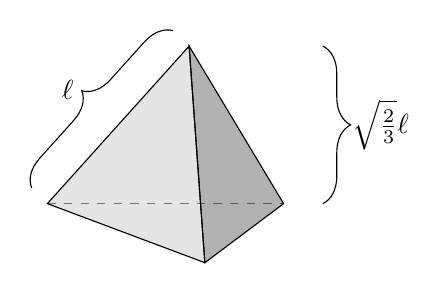
\begin{tikzpicture}
\draw (0,0) coordinate(a0);
\draw (3,0) coordinate(a1);
\draw (2,-.75) coordinate(a2);
\draw (1.8,2.) coordinate(a3);
\draw[dashed, gray] (a0)--(a1);
\draw[fill, fill opacity=0.3] (a2)--(a3)--(a1)--cycle;
\draw[fill, fill opacity=0.1] (a0)--(a3)--(a2)--cycle;
\draw[decorate, decoration={brace, amplitude=10pt}] (-.2,0.2)--(1.6,2.2) node[midway, above left, xshift=-7pt]{$\ell$};
\draw[decorate, decoration={brace, amplitude=10pt, mirror}] (3.5,0)--(3.5,2) node[midway,  right, xshift=7pt]{$\sqrt{\frac{2}{3}}\ell$};

\end{tikzpicture}
\end{center}
\end{question}
\begin{hint}
If you take horizontal slices (parallel to one face), they will all be equilateral triangles.

Be careful not to confuse the height of a \emph{triangle} with the height of the tetrahedron.
\end{hint}
\begin{answer}
$\dfrac{\sqrt{2}}{12}\ell^3$
\end{answer}
\begin{solution}
We'll make horizontal slices, parallel to one of the faces of the tetrahedron. Then our slices will be equilateral triangles, of varying sizes.

\begin{center}
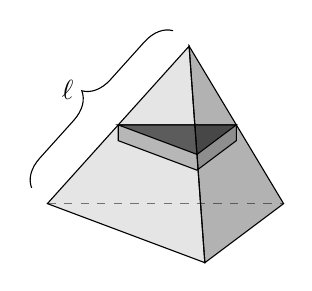
\begin{tikzpicture}
\draw (0,0) coordinate(a0);
\draw (3,0) coordinate(a1);
\draw (2,-.75) coordinate(a2);
\draw (1.8,2.) coordinate(a3);
\filldraw[fill opacity=0.5] (0.9,1)--(2.4,1)--(1.9,0.625)--cycle;
\filldraw[fill opacity=0.2] (0.9,1)--(0.9,0.8)--(1.9,0.425)--(2.4,.8)--(2.4,1)--cycle;
\draw[dashed, gray] (a0)--(a1);
\draw[fill, fill opacity=0.3] (a2)--(a3)--(a1)--cycle;
\draw[fill, fill opacity=0.1] (a0)--(a3)--(a2)--cycle;
\draw[decorate, decoration={brace, amplitude=10pt}] (-.2,0.2)--(1.6,2.2) node[midway, above left, xshift=-7pt]{$\ell$};
\end{tikzpicture}
\end{center}



 For the sake of ease, as in Example \eref{CLP101}{eg:VOLa} of the CLP-2 text,
we picture the tetrahedron perched on a tip, one base horizontal on top.

%Note that the height of an equilateral triangle with side-length $\ell$ is $\sqrt{\frac{2}{3}}\ell$ (which we find using the Pythagorean Theorem). Then at height $y$, the length of the side of an equilateral triangular cross-section is $\frac{2}{\sqrt{3}}y$, and its area is $\frac{1}{2}y\left(\frac{2}{\sqrt{3}}y\right)=\frac{y^2}{\sqrt{3}}$.
\begin{center}
\begin{tikzpicture}
\YEaaxis{3}{3}{1}{5}
\fill[fill opacity=0.1] (-1.84,2.8)--(0,3.3)--(1.84,2.8)--cycle;

\draw[thick](-1.2,3.8)-- (-2.5,3.8)--(0,0)--(2.5,3.8)--(-.2,3.8);
\YEycoord{3}{y}
\YEycoord{4.08}{\sqrt{\frac{2}{3}}\ell}
\YExcoord{2.5}{\frac{\ell}{2}}
\YExcoord{-2.5}{-\frac{\ell}{2}}
%\draw (-1.84,3)--(-.75,3) (.3,3)--(1.84,3);
%\draw (0,0)--(2.5,3.9)--(2.5,4.08);
\draw (-2.5,3.8)-- (0,4.5)--(2.5,3.8);
\end{tikzpicture}
\end{center}

Notice our slice forms the horizontal top of a smaller tetrahedron. The horizontal top of the full tetrahedron has side length $\ell$, which is
             $\sqrt{\frac{3}{2}}$ times the height of the full tetrahedron. Our slice
             is the horizontal top of a tetrahedron of height $y$ and so has side length  $\sqrt{\frac{3}{2}}y$. An equilateral triangle with side length $L$ has base $L$ and height
              $\frac{\sqrt{3}}{2}L$, and hence area $\frac{\sqrt{3}}{4}L^2$.
             So, the area of our slice with side length $\sqrt{\frac{3}{2}}y$ is
\[A = \frac{\sqrt{3}}{4}\left(\sqrt{\frac{3}{2}}y\right)^2 = \frac{3\sqrt{3}}{8}y^2\]

So, the volume of a tetrahedron with side length $\ell$ is:
\begin{align*}
\mbox{Volume}&=\int_0^{\sqrt{\frac{2}{3}}\ell}\frac{3\sqrt{3}}{8}y^2\ \dee{y}\\
&=\frac{\sqrt{3}}{8}\cdot \left(\sqrt{\frac{2}{3}}\ell\right)^3=\frac{\sqrt{2}}{12}\ell^3
\end{align*}



\emph{You were given the height of a tetrahedron, but for completeness we calculate it here.}


Draw a line starting at one tip, and dropping straight down to the middle of the opposite face. It forms a right triangle with one edge of the tetrahedron, and a line from the middle of the face to the corner.


\begin{center}
\begin{tikzpicture}[scale=1.5]
\draw (0,0) coordinate(a0);
\draw (3,0) coordinate(a1);
\draw (2,-.75) coordinate(a2);
\draw (1.8,2.) coordinate(a3);
\draw[dashed, gray] (a0)--(a1);
\draw[fill, fill opacity=0.3] (a2)--(a3)--(a1)--cycle;
\draw[fill, fill opacity=0.1] (a0)--(a3)--(a2)--cycle;
\draw[decorate, decoration={brace, amplitude=10pt}] (-.2,0.2)--(1.6,2.2) node[midway, above left, xshift=-7pt]{$\ell$};
\draw[thick, densely dotted] (1.8,2)--(1.7,-.3)--(a0);
\draw(1.7,-.3) node[vertex, label=below:$c$]{};
\draw (a0) node[left]{$A$};
\draw (a1) node[right]{$C$};
\end{tikzpicture}
\end{center}

We know the length of the hypotenuse of this right triangle (it's $\ell$), so if we know the length of its base (labeled $Ac$ in the diagram), we can figure out its third side, the height of our tetrahedron. Note by using the Pythagorean theorem, we see that the height of an equilateral triangle with edge length $\ell$ is $\sqrt{\frac{3}{2}}\ell$.

Here is a sketch of the base of the pyramid:

\begin{center}
\begin{tikzpicture}
\draw node[vertex]{};
\foreach \x in {0,1,2}{
	\draw (0,0) + (30+120*\x:3cm) node[vertex](v\x){};}
\draw (v1) node[left]{$A$};
\draw (v0) node[right]{$C$};
\draw (v0)--(v1)--(v2)--(v0);
\draw (v0)--(v2) coordinate[midway, label=right:{$B$}](m0){};
\draw (v1)--(v0) coordinate[midway, label=above:{$b$}](m2){};
\draw (v1)--(m0);
\draw (0,0)--(m2);
\draw  node[below]{$c$};
\draw  (-1,-1.5) node[below]{$\ell$};
\end{tikzpicture}
\end{center}

The triangles $ABC$ and $Abc$ are similar (since $b$ and $B$ are right angles, and also $A$ has the same angle in both). Therefore,
\begin{align*}
\frac{{Ac}}{{Ab}}&=\frac{{AC}}{{AB}}\\
\frac{Ac}{\ell/2}&=\frac{\ell}{\sqrt{3}\ell/2}\\
Ac&=\frac{1}{\sqrt{3}}\ell
\end{align*}

With this in our pocket, we can find the height of the tetrahedron: $\sqrt{\ell^2 - \left(\frac{1}{\sqrt{3}}\ell\right)^2} =\sqrt{\frac{2}{3}}\ell$.


\end{solution}


%%%%%%%%%%%%%%%%%%
\subsection*{\Procedural}
%%%%%%%%%%%%%%%%%%

\begin{Mquestion}[2016Q3] %% 5
Let $a>0$ be a constant. Let $R$ be the finite region bounded by the
graph of $y=1+\sqrt{x}e^{x^2}$, the line $y=1$, and the line $x=a$. Using
vertical slices, find the volume generated when $R$ is rotated about the line $y=1$.
\end{Mquestion}

\begin{hint}
Sketch the region.
\end{hint}

\begin{answer}
$\displaystyle\frac{\pi}{4}\Big(e^{2a^2}-1\Big)$
\end{answer}

\begin{solution}
Let $f(x)=1+\sqrt{x}e^{x^2}$.
On the vertical slice a distance $x$ from the $y$-axis,
sketched in the figure below, $y$ runs from $1$ to $f(x)$. Upon rotation
about the line $y=1$, this thin slice sweeps out a thin disk of thickness
$\dee{x}$ and radius $f(x)-1$ and hence of volume $\pi[f(x)-1]^2\,\dee{x}$.
The full volume generated (for any fixed $a>0$) is
\begin{align*}
\int_0^a\pi[f(x)-1]^2\,\dee{x}
=\pi\int_0^axe^{2x^2}\,\dee{x}.
\end{align*}
Using the substitution $u=2x^2$, so that $\dee{u}=4x\,\dee{x}$:
\begin{align*}
\text{Volume} = \pi\int_0^{2a^2}e^u\,\frac{\dee{u}}{4}
=\frac{\pi}{4}e^u\Big|_0^{2a^2}
=\frac{\pi}{4}\Big(e^{2a^2}-1\Big)
\qquad\qquad\smash{\raisebox{-0.4\height}{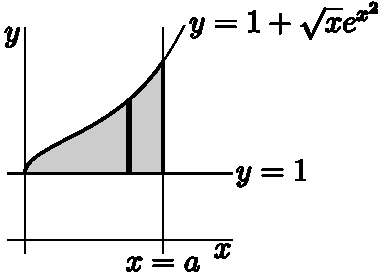
\includegraphics{OQ16_3_4b}}}
\end{align*}

\vspace{1cm}
Remark: we spent a good deal of time last semester developing highly accurate but time-consuming methods for sketching common functions. For the purposes of questions like this, we don't need a detailed picture of a function--broad outlines suffice. Notice that $\sqrt{x} > 0$ whenever $x>0$, and $e^{x^2}>0$ for all $x$. Therefore, $\sqrt{x}e^{x^2}$ is nonnegative over its entire domain, and so the graph $y=1+\sqrt{x}e^{x^2}$ is always the top function, above the bottom function $y=1$. That is the only information we needed to perform our calculation.
\end{solution}
%%%%%%%%%%%%%%%%%%%





\begin{question}[2014A] %% 7
Find the volume of the solid generated by rotating the finite
region bounded by $y = 1/x$ and $3x + 3y = 10$ about the $x$--axis.
\end{question}

\begin{hint}
Sketch the region first.
\end{hint}

\begin{answer}
$\pi\left[\dfrac{38}{3}-\dfrac{514}{3^4}\right] = \pi\dfrac{512}{81}$
\end{answer}

\begin{solution}

The curves $y=1/x$ and $3x+3y=10$, i.e. $y =\frac{10}{3}-x$ intersect
when
\begin{align*}
\frac{1}{x} = \frac{10}{3}-x
&\iff 3 = 10x-3x^2
\iff 3x^2-10x+3=0 \\
&\iff(3x-1)(x-3)=0 \\
&\iff x=3\,,\,\frac{1}{3}
\end{align*}

\smallskip
\centerline{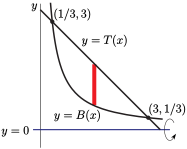
\includegraphics[scale=1.0]{OE14A_3}}
\smallskip

\noindent
When the region is rotated about the $x$--axis, the vertical strip
in the figure above sweeps out a washer with thickness $\dee{x}$,
outer radius $T(x)=\frac{10}{3}-x$ and inner radius $B(x)=\frac{1}{x}$.
This washer has volume
\begin{equation*}
\pi\big(T(x)^2- B(x)^2\big)\,\dee{x}
= \pi\Big(\frac{100}{9}-\frac{20}{3}x+x^2-\frac{1}{x^2}\Big)\,\dee{x}
\end{equation*}
Hence the volume of the solid is
\begin{align*}
\pi\int_{1/3}^3\Big(\frac{100}{9}-\frac{20}{3}x+x^2-\frac{1}{x^2}\Big)\,\dee{x}
&=\pi\Big[\frac{100x}{9}-\frac{10}{3}x^2+\frac{1}{3}x^3
              +\frac{1}{x}\Big]_{1/3}^3 \\
&=\pi\Big[\frac{38}{3}-\frac{514}{3^4}\Big] = \pi\frac{512}{81}
\end{align*}
\end{solution}
%%%%%%%%%%%%%%%%%%%


\begin{question}[2015A] %% 8
 Let $R$ be the region inside the circle $x^2 + (y-2)^2=1$. Let $S$ be the solid obtained by rotating $R$ about the $x$-axis.
\begin{enumerate}[(a)]
\item
 Write down an integral representing the volume of $S$.
\item
Evaluate the integral you wrote down in part (a).
\end{enumerate}
\end{question}

\begin{hint}
You can save yourself quite a bit of work by interpreting the integral
as the  area of a known geometric figure.
\end{hint}

\begin{answer} (a)
$8\pi\int_{-1}^1\sqrt{1-x^2}\,\dee{x}$
\qquad (b)
$ 4\pi^2$
\end{answer}

\begin{solution} (a)
The top and the bottom of the circle have equations
$y=T(x)=2+\sqrt{1-x^2}$ and $y=B(x) = 2-\sqrt{1-x^2}$, respectively.

\smallskip
\centerline{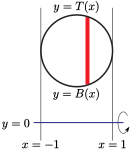
\includegraphics{OE15A_10}}
\smallskip

\noindent
When $R$ is rotated about the $x$--axis, the vertical strip of
$R$ in the figure above sweeps out a washer with thickness $\dee{x}$,
outer radius $T(x)$ and inner radius $B(x)$. This washer has
volume
\begin{equation*}
\null\hskip0.5in\pi\big(T(x)^2- B(x)^2\big)\,\dee{x}
= \pi\big(T(x)+ B(x)\big)\big(T(x)- B(x)\big)\,\dee{x}
= \pi\times 4\times 2\sqrt{1-x^2}\,\dee{x}
\end{equation*}
Hence the volume of the solid is
\begin{equation*}
8\pi\int_{-1}^1\sqrt{1-x^2}\,\dee{x}
\end{equation*}

\noindent (b)
Since $y=\sqrt{1-x^2}$ is equivalent to $x^2+y^2=1$, $y\ge 0$,
the integral is $8\pi$ times the area of the upper half
of the circle $x^2+y^2=1$ and hence is
$8\pi\times \frac{1}{2}\pi 1^2 = 4\pi^2$.


\end{solution}
%%%%%%%%%%%%%%%%%%%

\begin{question}[1996D] %% 9
 The region $R$ is the portion of the first quadrant which
is below the parabola $y^2=8x$ and above the hyperbola $y^2-x^2=15$.
\begin{enumerate}[(a)]
\item
Sketch the region $R$.
\item
Find the volume of the solid obtained by revolving $R$ about the $x$ axis.
\end{enumerate}
\end{question}

\begin{hint}
See Example \eref{CLP101}{eg:VOLe} in the
%\href{http://www.math.ubc.ca/%7Efeldman/m101/clp/clp_notes_101.pdf}{CLP 101 notes}.
CLP-2 text.
\end{hint}

\begin{answer} (a)
The region $R$ is the region
between the blue and red curves, with $3\le x\le 5$,  in the figures below.

\begin{center}
       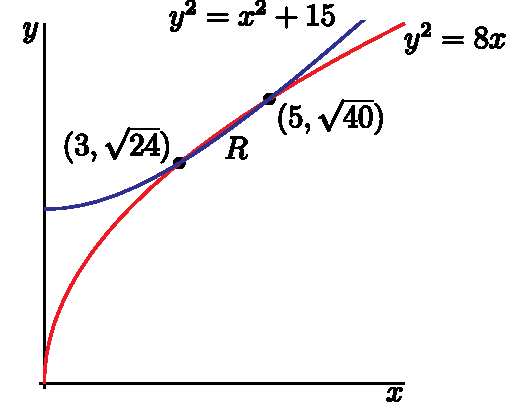
\includegraphics{graphE1}\qquad
       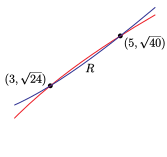
\includegraphics{graphE1b}
\end{center}

\noindent (b) $\frac{4}{3}\pi\approx 4.19$
\end{answer}

\begin{solution} (a)
The two curves intersect when $x$ obeys $8x=x^2+15$
or $x^2-8x+15=(x-5)(x-3)=0$. The points of intersection, in the first quadrant,
are $(3,\sqrt{24})$ and $(5, \sqrt{40})$. The region $R$ is the region
between the blue and red curves, with $3\le x\le 5$,  in the figures below.

\begin{center}
       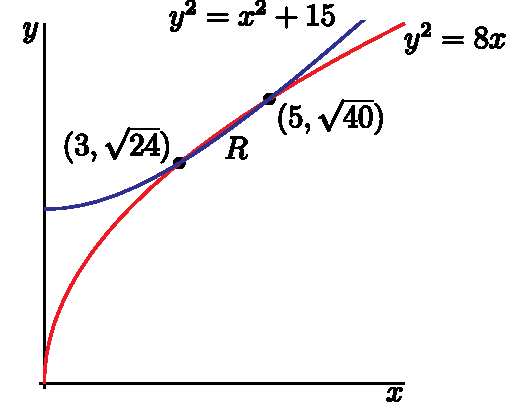
\includegraphics{graphE1}\qquad
       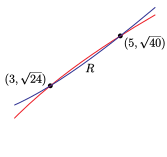
\includegraphics{graphE1b}
\end{center}

\item{}(b) The part of the solid with $x$ coordinate between $x$ and $x+\dee{x}$
is a ``washer'' shaped region with inner radius $\sqrt{x^2+15}$, outer
radius $\sqrt{8x}$ and thickness $\dee{x}$. The surface area of the washer is
$\pi(\sqrt{8x})^2 -\pi(\sqrt{x^2+15})^2=\pi(8x-x^2-15)$ and its volume is
$\pi(8x-x^2-15)\,\dee{x}$. The total volume is
\begin{align*}
\int_3^5 \pi(8x-x^2-15)\,\dee{x}
&=\pi\Big[4x^2-\frac{1}{3}x^3-15 x\Big]_3^5
=\pi\Big[100-\frac{125}{3}-75-36+9+45\Big] \\
&=\frac{4}{3}\pi\approx 4.19
\end{align*}

\end{solution}
%%%%%%%%%%%%%%%%%%%


\begin{Mquestion}[1996D] %% 10
 The region $R$ is bounded by $y=\log x$, $y=0$, $x=1$ and $x=2$.
(Recall that we are using $\log x$ to denote the logarithm of $x$ with
base $e$. In other courses it is often denoted $\ln x$.)
\begin{enumerate}[(a)]
\item
Sketch the region $R$.
\item
Find the volume of the solid obtained by revolving this region  about the $y$ axis.
\end{enumerate}
\end{Mquestion}

\begin{hint}
See Example \eref{CLP101}{eg rot yaxis} in the
%\href{http://www.math.ubc.ca/%7Efeldman/m101/clp/clp_notes_101.pdf}{CLP 101 notes}.
CLP-2 text.
\end{hint}

\begin{answer} (a)
The region $R$ is sketched below.

\begin{center}
       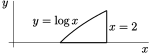
\includegraphics{graphE2l}
\end{center}

\noindent (b) $\pi\Big[4\log 2 - \frac{3}{2}\Big] \approx 3.998$
\end{answer}

\begin{solution} (a)
The region $R$ is sketched in the figure on the left below. (The bound $y=0$ renders the bound $x=1$ unnecessary, since the graph $y=\log x$ hits the $x$-axis when $x=1$.)

\begin{center}
       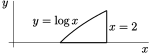
\includegraphics{graphE2l}\qquad
       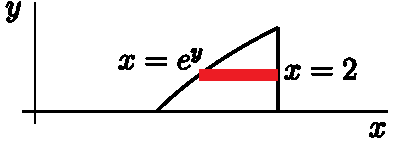
\includegraphics{graphE2r}
\end{center}

\noindent (b)
We'll use horizontal washers as in Example  \eref{CLP101}{eg rot yaxis}
of the %\href{http://www.math.ubc.ca/%7Efeldman/m101/clp/clp_notes_101.pdf}{CLP 101 notes}.
CLP-2 text.
 \begin{itemize}
\item We cut $R$ into thin horizontal  strips of height $\dee{y}$ as in
the figure on the right above.

\item When we rotate $R$ about the $y$--axis, i.e. about the line $x=0$,
each strip sweeps out a thin washer
\begin{itemize}
\item whose inner radius is $r_{in}= e^y$ and outer radius is $r_{out}=2$, and
\item whose thickness is $\dee{y}$ and hence
\item whose volume $\pi(r_{out}^2 - r_{in}^2)\dee{y} = \pi\big(4-e^{2y}\big)\dee{y}$.
\end{itemize}
\item As our bottommost strip is at $y=0$ and our topmost
strip is at $y=\log 2$ (since at the top $x=2$ and $x=e^y$), the total
\begin{align*}
\text{Volume}
&= \int _0^{\log 2} \pi\big(4-e^{2y}\big)\ \dee{y}
=\pi\big[4y -e^{2y}/2\big]_0^{\log 2}
=\pi\Big[4\log 2 - 2 +\frac{1}{2}\Big] \\
&=\pi\Big[4\log 2 - \frac{3}{2}\Big]
\end{align*}
Using a calculator, we see this is approximately $3.998$.
\end{itemize}
\end{solution}
%%%%%%%%%%%%%%%%%%%

\begin{question}[2016Q3] %% 11
The finite region between the curves $y = \cos(\frac x2)$
and $y = x^2 - \pi^2$ is rotated about the line $y=-{\pi^2}$.
Using vertical slices (disks and/or washers), find the volume of
the resulting solid.
\end{question}

\begin{hint}
Sketch the region. To find where the curves intersect, look at where
$\cos(\frac x2)$ and $x^2 - \pi^2$  both have roots.
\end{hint}

\begin{answer}
 $\pi^2 + 8\pi^3 + \frac{8\pi^6}{5}$
\end{answer}

\begin{solution}
Here is a sketch of the curves $y = \cos(\frac x2)$ and $y = x^2 - \pi^2$.

\begin{center}
       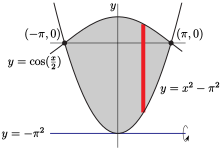
\includegraphics{OQ16_3_4}
\end{center}

By inspection, the curves meet at $x = \pm {\pi}$ where both $\cos(\frac x2)$  and
$x^2 - \pi^2$ take the value zero.
We'll use vertical washers as specified in the question.
 \begin{itemize}
\item We cut the specified region into thin vertical strips of
width $\dee{x}$ as in the figure above.

\item When we rotate about the line $y=-\pi^2$,
each strip sweeps out a thin washer
\begin{itemize}
\item whose inner radius is $r_{in}= (x^2 - {\pi^2} ) - ( {-} {\pi^2} )=x^2$
and outer radius is $r_{out}=\cos(\frac x2) - ( {-} {\pi^2})
=\cos(\frac x2) +\pi^2 $, and
\item whose thickness is $\dee{x}$ and hence
\item whose volume
    $\pi(r_{out}^2 - r_{in}^2)\dee{x}
        =  \pi\big( {(\cos(\frac x2) +\pi^2)}^2 - {(x^2)}^2\big)\dee{x}$.
\end{itemize}
\item As our leftmost strip is at $x=-\pi$ and our rightmost
strip is at $x=\pi$,
\end{itemize}
the total volume is
\begin{align*}
  &\pi \int_{-\pi}^{\pi}
         \left(  \cos^2 (\tfrac x2) +2{\pi^2}\cos (\tfrac x2) +{\pi^4} -x^4\right)\,\dee{x} \\
 &\hskip0.5in = \pi \int_{-\pi}^{\pi}
         \left(\frac{1+\cos(x)}{2} +2{\pi^2}\cos (\tfrac x2) +{\pi^4} -x^4\right)\,\dee{x}
         \intertext{Because the integrand is even,}
 &\hskip0.5in = 2\pi \int_0^{\pi}
         \left(\frac{1+\cos(x)}{2} +2{\pi^2}\cos (\tfrac x2) +{\pi^4} -x^4\right)\,\dee{x} \\
 &\hskip0.5in = {2\pi \left[ \frac{1}{2}x + \frac{1}{2}\sin(x)
          + 4{\pi^2}\sin (\tfrac x2)  +{\pi^4} x -\frac{1}{5}x^5   \right]} _0^\pi\\
 &\hskip0.5in = 2\pi \left[\frac{\pi}{2} + 0 + 4{\pi^2} +{\pi^5} - \frac{\pi^5}{5} \right] \\
 &\hskip0.5in = {\pi^2} + 8\pi^3 + \frac{8\pi^6}{5}
\end{align*}
We used the fact that the integrand is an even function and the interval of integration $[-\pi, \pi]$ is symmetric, but one can also compute directly.

%\centerline{
%\begin{tikzpicture}
%\draw[domain=-2.00:2.00,dashed] plot (\x,{cos(\x r)});
%\draw[domain=-2.00:2.00,dashed] plot (\x,{\x*\x-2.47});
%\draw[domain=-1.57:1.57] plot (\x,{cos(\x r)});
%\draw[domain=-1.57:1.57] plot (\x,{\x*\x-2.47});
%\draw[dashed] (-2.5,-2.47) -- (2.5,-2.47);
%\node at (-1.5,-2.8) {$y = -\pi^2$};
%\draw (+1.57,0) -- (+1.57,-0.2) node[below] {${\pi}$};
%\draw (-1.57,0) -- (-1.57,-0.2) node[below] {$-{\pi}$};
%\draw[ultra thick,->] (-2.5,0) -- (2.5,0);
%\draw[ultra thick,->] (0,-3.5) -- (0,3);
%\end{tikzpicture}
%}
\end{solution}
%%%%%%%%%%%%%%%%%%%


\begin{Mquestion}[1997D] %% 12
The solid $V$ is 2 meters high and has square horizontal
cross sections. The length of the side of the square cross section at height
$x$ meters above the base is $\frac{2}{1+x}$ m. Find the volume
of this solid.
\end{Mquestion}

\begin{hint}
See Example \eref{CLP101}{eg:VOLb} in the
%\href{http://www.math.ubc.ca/%7Efeldman/m101/clp/clp_notes_101.pdf}{CLP 101 notes}.
CLP-2 text.
\end{hint}

\begin{answer}
$\dfrac{8}{3}$
\end{answer}

\begin{solution}
As in Example \eref{CLP101}{eg:VOLb} of the
%\href{http://www.math.ubc.ca/%7Efeldman/m101/clp/clp_notes_101.pdf}{CLP 101 notes}.
CLP-2 text notes, we slice $V$  into thin horizontal ``square pancakes''.

\begin{itemize}
\item We are told that the pancake at height $x$ is a square
of side $\frac{2}{1+x}$ and so
\item has cross-sectional area $\big(\frac{2}{1+x}\big)^2$ and
thickness $\dee{x}$ and hence
\item has volume $\big(\frac{2}{1+x}\big)^2\dee{x}$.
\end{itemize}
\noindent Hence the volume of $V$ is
$$
\int_0^2{\Big[\frac{2}{1+x}\Big]}^2\,\dee{x}
=\int_1^3\frac{4}{u^2}\,\dee{u}
=4\frac{u^{-1}}{-1}\bigg|_1^3
=-4\Big[\frac{1}{3}-1\Big]
=\frac{8}{3}
$$
We made the change of variables $u=1+x$, $\dee{u}=\dee{x}$.
\end{solution}
%%%%%%%%%%%%%%%%%%%

\begin{question}[1998A] %% 13
Consider a solid whose base is the finite portion of the
$xy$--plane bounded by the curves $y=x^2$ and $y=8-x^2$. The cross--sections
perpendicular to the $x$--axis are squares with one side in the $xy$--plane.
Compute the volume of this solid.
\end{question}

\begin{hint}
See Example \eref{CLP101}{eg:VOLb} in the
%\href{http://www.math.ubc.ca/%7Efeldman/m101/clp/clp_notes_101.pdf}{CLP 101 notes}.
CLP-2 text. Imagine cross-sections with shadow parallel to the $y$-axis, sticking straight out of the $xy$-plane.
\end{hint}

\begin{answer}
 $\dfrac{256\times 8}{15}=136.5\dot3$
\end{answer}

\begin{solution}
Here is a sketch of the base region.

\begin{center}
       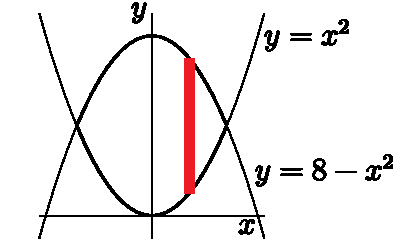
\includegraphics{graphE98A_7}
\end{center}

\noindent
Consider the thin vertical cross--section resting on the heavy red
line in the figure above. It has thickness $\dee{x}$. Its face is a square
whose side runs from $y=x^2$ to $y=8-x^2$, a distance of $8-2x^2$. So the
face has area ${(8-2x^2)}^2$ and the slice has volume ${(8-2x^2)}^2\,\dee{x}$. The two
curves cross when $x^2=8-x^2$, i.e. when $x^2=4$ or $x=\pm 2$. So $x$ runs
from $-2$ to $2$ and the total volume is
\begin{align*}
\int_{-2}^{2}{(8-2x^2)}^2\,\dee{x}&=2\int_0^2 4{(4-x^2)}^2\,\dee{x}
=8\int_0^2\big[16-8x^2+x^4\big]\,\dee{x}\cr
&=8\Big[16\times 2-\frac{8}{3}2^3+\frac{1}{5}2^5\Big]
=\frac{256\times 8}{15}=136.5\dot3
\end{align*}
In the first simplification step, we used the fact that our integrand was even, but we also could have finished our computation without this step.
\end{solution}
%%%%%%%%%%%%%%%%%%%

\begin{Mquestion}[2001D] %% 14
A frustrum of a right circular cone (as shown below) has
height $h$. Its base is a circular disc with radius $4$ and its top is
a circular disc with radius $2$. Calculate the volume of the frustrum.
\begin{center}
       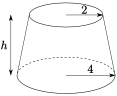
\includegraphics{OE01D_4b}
\end{center}
\end{Mquestion}

\begin{hint}
See Example \eref{CLP101}{eg:VOLa} in the
%\href{http://www.math.ubc.ca/%7Efeldman/m101/clp/clp_notes_101.pdf}{CLP 101 notes}.
CLP-2 text.
\end{hint}

\begin{answer}
$\dfrac{28}{3}\pi h$
\end{answer}

\begin{solution}
Slice the frustrum into horizontal discs. When the disc is a distance
$t$ from the top of the frustrum it has radius $2+2t/h$. Note that as $t$
runs from $0$ (the top of the frustrum) to $t=h$ (the bottom of the frustrum)
the radius $2+2t/h$ increases linearly from $2$ to $4$.
\begin{center}
       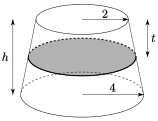
\includegraphics{OE01D_4}
\end{center}
 Thus the disk has volume $\pi \big(2+2t/h\big)^2 \dee{t}$. The total volume of the
frustrum is
\begin{align*}
\pi\int_0^h \big(2+2t/h\big)^2 \dee{t}
=4\pi\int_0^h \big(1+t/h\big)^2 \dee{t}
=4\pi\left[\frac{(1+t/h)^3}{3/h}\right]_0^h
=\frac{4}{3}\pi h\times 7
=\frac{28}{3}\pi h
\end{align*}

Remark: we could also solve this problem using the formula for the volume of a cone. Using similar triangles, the frustrum in question is shaped like a right circular cone of height $2h$ and base radius 4 (and hence of volume $\dfrac{1}{3}\pi(4^2)(2h)$), but missing its top, which is a right circular cone of height $h$ and base radius $2$ (and hence volume $\dfrac{1}{3}\pi(2^2)h$). So, the volume of the frustrum is $\dfrac{1}{3}\pi(4^2)(2h) - \dfrac{1}{3}\pi(2^2)h = \dfrac{28}{3}\pi h$.
\end{solution}
%%%%%%%%%%%%%%%%%%%







%%%%%%%%%%%%%%%%%%
\subsection*{\Application}
%%%%%%%%%%%%%%%%%%

\begin{question}
The shape of the earth is often approximated by an oblate spheroid, rather than a sphere. An \emph{oblate spheroid} is formed by rotating an ellipse about its \emph{minor axis} (its shortest diameter).
\begin{enumerate}[(a)]
\item Find the volume of the oblate spheroid obtained by rotating the upper (positive) half of the ellipse $(ax)^2+(by)^2=1$ about the $x$-axis, where $a$ and $b$ are positive constants with $a \geq b$.
\item Suppose\footnote{Earth Fact Sheet, NASA, \url{https://nssdc.gsfc.nasa.gov/planetary/factsheet/earthfact.html}, accessed 2 July 2017} the earth has radius at the equator of 6378.137  km, and radius at the poles of 6356.752 km. If we model the earth as an oblate spheroid formed by rotating the upper half of the ellipse $(ax)^2+(by)^2=1$ about the $x$-axis, what are $a$ and $b$?
\item What is the volume of this model of the earth? (Use a calculator.)
\item Suppose we had calculated the volume of the earth by modelling it as a sphere with radius $6378.137$ km. What would our absolute and relative errors be, compared to our oblate spheroid calculation?
\end{enumerate}
\end{question}
\begin{hint}
(a) Don't be put off by phrases like ``rotating an ellipse about its minor axis." This is the same kind of volume you've been calculating all section.\\
(b) Hopefully, you sketched the ellipse in part (a). What was its smallest radius? Its largest? These correspond to the polar and equitorial radii, respectively.\\
(c) Combine your answers from (a) and (b).\\
(d) Remember that the absolute error is the absolute difference of your two results--that is, you subtract them and take the absolute value. The relative error is the absolute error divided by the actual value (which we're taking, for our purposes, to be your answer from (c)). When you take the relative error, lots of terms will cancel, so it's easiest to not use a calculator till the end.
\end{hint}
\begin{answer}
(a) $\dfrac{4\pi}{3b^2a}$ cubic units \qquad
(b) $a = \dfrac{1}{6356.752}$ and $b=\dfrac{1}{6378.137}$\\[5pt]
(c) Approximately $ 1.08321\times 10^{12} ~\mathrm{km}^3$, \quad or \quad
$ 1.08321\times 10^{21}~ \mathrm{m}^3$\\[5pt]
(d) Absolute error is about $3.64\times 10^{9}~ \mathrm{km}^3$, and relative error is about
$0.00336$, or $0.336\%$.
\end{answer}
\begin{solution}
(a)

We'll want to start by graphing the upper half of the ellipse $(ax)^2+(by)^2=1$. Its intercepts will be enough to get us an idea: $(0,\frac{1}{b})$ and $(\pm\frac{1}{a},0)$:
\begin{center}
\begin{tikzpicture}
\YEaaxis{3.5}{3.5}{1}{4.25}
\YExcoord{3}{\frac{1}{a}}
\YExcoord{-3}{-\frac{1}{a}}
\draw (.2,4)--(-1,4) node[left]{$\frac{1}{b}$};
\draw[thick, blue] plot[domain=-3:3, samples=100](\x,{4*sqrt(1-(\x/3)^2)});
\draw[blue] (3,3) node[right]{$y=\frac{1}{b}\sqrt{1-(ax)^2}$};
\end{tikzpicture}
\end{center}

We note a few things at the outset: first, since $a \geq b$, then $\frac{1}{a} \leq \frac{1}{b}$, so indeed the $x$-axis is the minor axis. That is, we're rotating about the proper axis to create an oblate spheroid.

Second, if we solve our equation for $y$, we get $y=\frac{1}{b}\sqrt{1-(ax)^2}$. (Since we only want the upper half of the ellipse, we only need to consider the positive square root.)

Now, we have a standard volume-of-revolution problem. We make vertical slices, of width $\dee{x}$ and height $y=\frac{1}{b}\sqrt{1-(ax)^2}$. When we rotate these slices about the $x$-axis, they form thin disks of volume $\pi\left[\frac{1}{b}\sqrt{1-(ax)^2}\right]^2\dee{x}$\ . Since $x$ runs from $-\frac{1}{a}$ to $\frac{1}{a}$, the volume of our oblate spheroid is:
\begin{align*}
\mbox{Volume}&=\int_{-\frac{1}{a}}^{\frac{1}{a}} \pi \left[\frac{1}{b}\sqrt{1-(ax)^2}\right]^2\dee{x}\\
&=\frac{\pi}{b^2}\int_{-\frac{1}{a}}^{\frac{1}{a}} 1-(ax)^2\ \dee{x}\\
&=\frac{2\pi}{b^2}\int_{0}^{\frac{1}{a}} 1-(ax)^2\ \dee{x}&\mbox{(even function)}\\
&=\frac{2\pi}{b^2}\left[x - \frac{a^2x^3}{3}\right]_{0}^{\frac{1}{a}}\\
&=\frac{2\pi}{b^2}\left[\frac{1}{a} - \frac{1}{3a} \right] = \frac{4\pi}{3b^2a}
\end{align*}

(b) As we saw in the sketch from part (a), the shortest radius of the ellipse is $\frac{1}{a}$, while the largest is $\frac{1}{b}$. So, $\frac{1}{a} = 6356.752$, and $\frac{1}{b} = 6378.137$. That is, $a = \dfrac{1}{6356.752}$ and $b=\dfrac{1}{6378.137}$.

Note $a \geq b$, as specified in part (a).

(c) Combining our answers from (a) and (b), the volume of an oblate spheroid with approximately the same dimensions as the earth is:
\begin{align*}
\frac{4\pi}{3b^2a} &= \frac{4\pi}{3}\left(\frac{1}{b}\right)^2\left(\frac{1}{a}\right)\\
&=\frac{4\pi}{3}\left(6378.137\right)^2\left(6356.752\right)\\
&\approx 1.08321\times 10^{12} \quad\mathrm{km}^3\\
&\approx 1.08321\times 10^{21} \quad\mathrm{m}^3
\end{align*}

(d) A sphere of radius 6378.137 has volume
\begin{align*}
&\dfrac{4}{3}\pi\left(6378.137\right)^3
\intertext{So, our absolute error is:}
&\left|\frac{4\pi}{3}\left(6378.137\right)^2\left(6356.752\right) - \dfrac{4}{3}\pi\left(6378.137\right)^3 \right|\\
=&\frac{4\pi}{3}\left(6378.137\right)^2\big|6356.752 - 6378.137\big|\\
=&\frac{4\pi}{3}\left(6378.137\right)^2(21.385)\\
\approx&~3.64 \times 10^{9}~\mathrm{km}^3
\intertext{And our relative error is:}
\frac{\mbox{abs error}}{\mbox{actual value}}&=\frac{\frac{4\pi}{3}\left(6378.137\right)^2\big|6356.752 - 6378.137\big|}{\frac{4\pi}{3}\left(6378.137\right)^2\left(6356.752\right)}\\
&=\frac{\big|6356.752 - 6378.137\big|}{6356.752}\\
&=\frac{6378.137}{6356.752}-1\\
&\approx ~0.00336
\end{align*}
That is, about $0.336\%$, or about one-third of one percent.
\end{solution}
%%%%%%%%%%%%%%%%%%%%%%%
\begin{question}[2012A] %%15
Let $R$ be the bounded region that lies between the curve
$y = 4 - (x - 1)^2$ and the line $y = x + 1$.
\begin{enumerate}[(a)]
\item
Sketch $R$ and find its area.
\item
Write down a definite integral giving the volume of the region
obtained by rotating $R$ about the line $y = 5$. \emph{Do not evaluate
this integral.}
\end{enumerate}
\end{question}

\begin{hint}
To find the points of intersection, set $4-(x-1)^2=x+1$.
\end{hint}

\begin{answer} (a)
$\dfrac{9}{2}$
\qquad(b)
$
\pi\displaystyle\int_{-1}^2
   \big[{\big(4-x\big)}^2-{\big(1+(x-1)^2\big)}^2\big]\,\dee{x}
$
\end{answer}

\begin{solution} (a)
The curve  $y = 4 - (x - 1)^2$ is an ``upside down parabola''
and line $y = x + 1$ has slope 1. They intersect at points $(x,y)$ which
satisfy both $y=x+1$ and $y=4-(x-1)^2$. That is, when $x$ obeys
\begin{align*}
x+1&=4-(x-1)^2\\
 x+1 &= 4 -x^2+2x-1\\
 x^2-x-2&=0 \\
 (x-2)(x+1)&=0\\
 x&=-1 \quad\mbox{or}\quad x=2
\end{align*}
Thus the intersection points are $(-1,0)$ and $(2,3)$.
Here is a sketch of $R$:

\begin{center}
       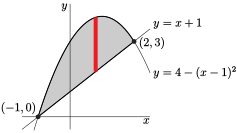
\includegraphics{OE12A_2a}
\end{center}

The red strip in the sketch above runs from $y=x+1$  to $y=4-(x-1)^2$
and so has area $[4-(x-1)^2 -(x+1)]\,\dee{x} = [2+x-x^2]\,\dee{x}$.
All together $R$ has
\begin{align*}
\text{Area}
&= \int_{-1}^2 \big[2+x-x^2\big]\ \dee{x} \\
&=\bigg[2x+\frac{x^2}{2}-\frac{x^3}{3}\bigg]_{-1}^2  \\
&=6+\frac{3}{2}-\frac{9}{3}=\frac{9}{2}
\end{align*}

\noindent (b)
We'll use vertical washers as in Example  \eref{CLP101}{eg:VOLe}
of the CLP-2 text. Note that the highest point achieved by $y=4-(x-1)^2$ is $y=4$, so rotating around the line $y=5$ causes no unexpected problems.

\begin{center}
       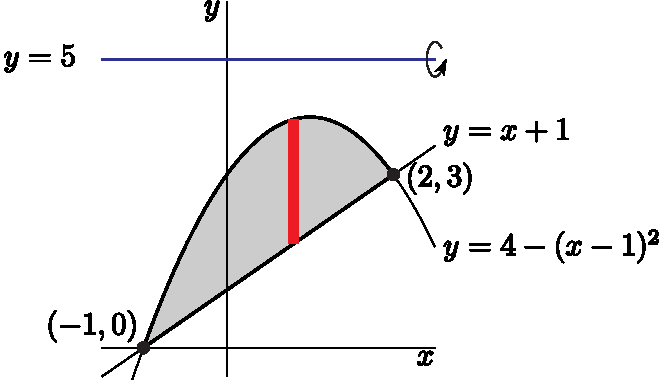
\includegraphics{OE12A_2b}
\end{center}

 \begin{itemize}
\item We cut $R$ into thin vertical strips of width $\dee{x}$ like the red
strip in the figure  above.

\item When we rotate $R$ about the horizontal line $y=5$,  each
strip  sweeps out a thin washer
\begin{itemize}
\item
whose inner radius is $r_{in}=5-[4-(x-1)^2]=1+(x-1)^2$, and
\item
whose outer radius is $r_{out}= 5-[x+1]=4-x$ and
\item
whose thickness is $\dee{x}$ and hence
\item
whose volume is
$\pi\big[r_{out}^2-r_{in}^2\big]\,\dee{x}
=\pi\big[{\big(4-x\big)}^2-{\big(1+(x-1)^2\big)}^2\big]\,\dee{x}$

\end{itemize}
\item As our leftmost strip is at $x=-1$ and our rightmost
strip is at $x=2$, the total
\begin{align*}
{\rm Volume} &= \pi\int_{-1}^2
   \big[{\big(4-x\big)}^2-{\big(1+(x-1)^2\big)}^2\big]\,\dee{x}
\end{align*}
\end{itemize}

\end{solution}
%%%%%%%%%%%%%%%%%%%


\begin{question}[M121 1999A]
 Let $\cR=\big\{(x,y)\ :\ (x-1)^2+y^2\le 1\text{
and } x^2+(y-1)^2\le 1\ \big\}$.
\begin{enumerate}[(a)]
\item
Sketch $\cR$ and find its area.
\item
 If $\cR$ rotates around the $y$--axis, what volume is generated?
\end{enumerate}
\end{question}

\begin{hint}
You can somewhat simplify your calculations in part (a) (but not part (b)) by using the fact that $\cR$ is symmetric about the line $y=x$.

When you're solving an equation for $x$, be careful about your signs: $x-1$ is negative.
\end{hint}

\begin{answer} (a)
$\dfrac{\pi}{2}-1$
\qquad(b)
$\dfrac{\pi^2}{2}-\pi\approx 1.793$
\end{answer}

\begin{solution} (a)
The curves  $(x-1)^2+y^2 = 1$ and  $x^2+(y-1)^2 = 1$
are circles of radius $1$ centered on $(1,0)$ and $(0,1)$ respectively.
Both circles pass through $(0,0)$ and $(1,1)$. They are sketched below.

\begin{center}
       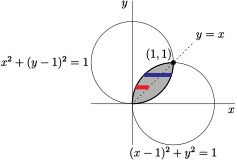
\includegraphics{E121_99D_8a}
\end{center}

\noindent The region $\cR$ is symmetric about the line $y=x$, so the area
of $\cR$ is twice the area of the part of $\cR$ to the left of the line $y=x$.
The red strip in the sketch above runs from  the edge of the lower circle to $x=y$.
So, given a value of $y$ in $[0,1]$, we need to find the corresponding value of $x$ along the circle. We solve $(x-1)^2+y^2=1$ for $x$, keeping in mind that $0 \leq x\leq 1$:
\begin{align*}
(x-1)^2+y^2&=1\\
(x-1)^2&=1-y^2\\
|x-1|&=\sqrt{1-y^2}\\
1-x&=\sqrt{1-y^2}\\
x&=1-\sqrt{1-y^2}
\intertext{Now, we calculate:}
\text{Area}
&= 2\int_0^1 \big[y-\big(1-\sqrt{1-y^2}\big)\big]\ \dee{y} \\
&=2\left\{ \int_0^1 y-1\ \dee{y} + \int_0^1 \sqrt{1-y^2}\ \dee{y} \right\}\\
&=2\Big\{\Big[\frac{y^2}{2}-y\Big]_0^1 +\int_0^1\sqrt{1-y^2}\ \dee{y}\Big\} \\
&=\frac{\pi}{2}-1
\end{align*}
Here the integral  $\int_0^1\sqrt{1-y^2}\ \dee{y}$ was evaluated simply as the area
of one quarter of a cicular disk of radius $1$. It can also be evaluated by substituting
$y=\sin\theta$, a technique we'll learn more about in Section~\eref{CLP101}{sec trigsub}
of the CLP-2 text.

\noindent (b)
We'll use horizontal washers as in Example  \eref{CLP101}{eg rot yaxis}
of the %\href{http://www.math.ubc.ca/%7Efeldman/m101/clp/clp_notes_101.pdf}{CLP 101 notes}.
 in the CLP-2 text.
 \begin{itemize}
\item We cut $\cR$ into thin horizontal  strips of width $\dee{y}$ like the blue
strip in the figure  above.

\item When we rotate $\cR$ about the $y$--axis,  each strip
sweeps out a thin washer
\begin{itemize}
\item
whose inner radius is $r_{in}=1-\sqrt{1-y^2}$, and
\item
whose outer radius is $r_{out}= \sqrt{1-(y-1)^2}$ and
\item
whose thickness is $\dee{y}$ and hence
\item
whose volume is
\begin{align*}
&\pi\big[{\big(\sqrt{1-(y-1)^2}\big)}^2-{\big(1-\sqrt{1-y^2}\,\big)}^2\big]\,\dee{y}\\
=&\pi \big[  1 - (y-1)^2       -1 + 2\sqrt{1-y^2} - (1-y^2)   \big]\\
=&2\pi\big[\sqrt{1-y^2}+y-1\big]\,\dee{y}\end{align*}

\end{itemize}
\item As our bottommost strip is at $y=0$ and our topmost
strip is at $y=1$, the total
\begin{align*}
{\rm Volume} &= 2\pi\int_{0}^1\big[\sqrt{1-y^2}+y-1\big]\ \dee{y}
= 2\pi\Big[\frac{\pi}{4}+\frac{1}{2}-1\Big]\\
&=\frac{\pi^2}{2}-\pi\approx 1.793
\end{align*}
Here, we again used that $\int_{0}^1 \sqrt{1-y^2}\ dy$ is the area of a quarter
circle of radius one, and we used a calculator to approximate the final answer.
\end{itemize}

\end{solution}
%%%%%%%%%%%%%%%%%%%

\begin{Mquestion}[1997A]
Let $\cR$ be the plane region bounded by $x=0,\ x=1,\ y=0$
and $y=c\sqrt{1+x^2}$, where $c\ge 0$ is a constant.
\begin{enumerate}[(a)]
\item
Find the volume $V_1$ of the solid obtained by revolving
$\cR$ about the $x$--axis.
\item
Find the volume $V_2$ of the solid obtained by revolving
$\cR$ about the $y$--axis.
\item
 If $V_1=V_2$, what is the value of $c$?
\end{enumerate}
\end{Mquestion}

\begin{hint}
The mechanically easiest way to answer part (b) uses the method of cylindrical
shells, which we have not covered.  The method of washers also works, but requires  you have enough patience and also
to have a good idea what $\cR$ looks like. So it is crucial to first sketch $\cR$.
Then be very careful in identifying the left end of your horizontal strips.
\end{hint}

\begin{answer} (a)
$V_1=\dfrac{4}{3}\pi c^2$
\qquad(b)
$V_2 =\dfrac{\pi\,c}{3}\big[4\sqrt{2}-2 \big] $
\qquad (c)
$c=0\text{ or }c=\sqrt{2}-\frac{1}{2}$
\end{answer}

\begin{solution}
Before we start, it will be useful to have a reasonable sketch of the graph $y=c\sqrt{1+x^2}$ over the interval $[0,1]$. Its endpoints are $(0,c)$ and $(1,c\sqrt{2})$. The function is entirely above the $x$-axis, which we need to know for part (a). For part (b), we need to know whether it is always increasing or not: when we're drawing horizontal strips, we need to know their endpoints, and if the function has ``humps," the right endpoint will not be simply the line $x=1$.

If you're comfortable noticing that $1+x^2$ increases as $x$ increases because we only consider nonnegative values of $x$, then you can also be confident that $\sqrt{1+x^2}$ is simply increasing. Alternately, we can consider the derivative:
\begin{align*}
\diff{}{x}\left\{c\sqrt{1+x^2}\right\}&=c\cdot \dfrac{1}{2\sqrt{1+x^2}}\cdot 2x = \dfrac{cx}{\sqrt{1+x^2}}
\end{align*}
Since we only consider positive values of $x$, this derivative is never negative, so the function is never decreasing. This gives us the following basic sketch:
\begin{center}
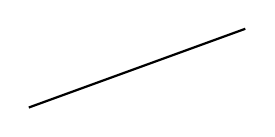
\begin{tikzpicture}
\YEaaxis{.5}{3}{.5}{3}
\YExcoord{2.5}{1}
\YEycoord{1}{c}
\draw[thick] (0,1)--(2.75,2) ;
\end{tikzpicture}
\end{center}

The figures in the solution below use a slightly more detailed rendering of our function, but so much accuracy is not necessary.

(a)
Let $\cV_1$ be the solid obtained by revolving
$\cR$ about the $x$--axis. The portion of $\cV_1$ with $x$--coordinate
between $x$ and $x+\dee{x}$ is obtained by rotating the red vertical strip in
the figure on the left below about the $x$--axis.
That portion is a disk of radius $c\sqrt{1+x^2}$ and thickness
$\dee{x}$. The volume of this disk is $\pi(c\sqrt{1+x^2})^2\dee{x}=\pi c^2 (1+x^2)\,\dee{x}$.
So the total volume of $\cV_1$ is
\begin{align*}
V_1=\int_0^1 \pi c^2 (1+x^2)\,\dee{x}
=\pi c^2\Big[x+\frac{x^3}{3}\Big]_0^1
=\frac{4}{3}\pi c^2
\end{align*}

\begin{center}
       
\includegraphics{graphE97_4l}\qquad\qquad
       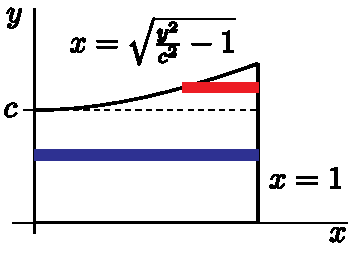
\includegraphics{graphE97_4r}
\end{center}


\noindent (b)
We'll use horizontal washers as in Example  \eref{CLP101}{eg rot yaxis}
of the %\href{http://www.math.ubc.ca/%7Efeldman/m101/clp/clp_notes_101.pdf}{CLP 101 notes}.
 in the CLP-2 text.
 \begin{itemize}
\item We cut $\cR$ into thin horizontal  strips of width $\dee{y}$ as in
the figure on the right above.

\item When we rotate $\cR$ about the $y$--axis, i.e. about the line $x=0$, each strip
sweeps out a thin washer
\begin{itemize}
\item
whose outer radius is $r_{out}=1$, and
\item
whose inner radius is $r_{in}= \sqrt{\frac{y^2}{c^2}-1}$ when $y\ge c\sqrt{1+0^2}=c$
(see the red strip in the figure on the right above),  and
whose inner radius is $r_{in}= 0$ when $y\le c$
(see the blue strip in the figure on the right above) and
\item
whose thickness is $\dee{y}$ and hence
\item
whose volume is
$\pi(r_{out}^2 - r_{in}^2)\dee{y} = \pi\big(2-\frac{y^2}{c^2}\big)\dee{y}$
when $y\ge c$ and  whose volume is
$\pi(r_{out}^2 - r_{in}^2)\dee{y} = \pi\,\dee{y}$
when $y\le c$ and

\end{itemize}
\item As our bottommost strip is at $y=0$ and our topmost
strip is at $y=\sqrt{2}\,c$ (since at the top $x=1$ and $y= c\sqrt{1+x^2}$), the total
\begin{align*}
V_2
&= \int _c^{\sqrt{2}\,c}  \pi\Big(2-\frac{y^2}{c^2}\Big)\dee{y}
+\int _ 0^c \pi\,\dee{y} \\
&=\pi{\Big[2y -\frac{y^3}{3c^2}\Big]}_c^{\sqrt{2}\,c} +\pi c\\
&=\pi\,c\Big[\frac{4\sqrt{2}}{3}-\frac{5}{3} \Big]+\pi c \\[0.05in]
&=\frac{\pi\,c}{3}\big[4\sqrt{2}-2 \big]
\end{align*}
\end{itemize}

\noindent (c)
We have $V_1=V_2$ if and only if
\begin{align*}
\frac{4}{3}\pi c^2&=\frac{\pi\,c}{3}\big[4\sqrt{2}-2 \big]  \\
4c^2&=c\left(4\sqrt{2}-2\right)\\
4c^2-c\left(4\sqrt{2}-2\right)&=0\\
4c\left(c - \left(\sqrt{2}-\frac{1}{2}\right)\right)&=0\\
c=0 \quad\mbox{or}\quad c&=\sqrt{2}-\frac{1}{2}
\end{align*}


\end{solution}
%%%%%%%%%%%%%%%%%%%

\begin{question}[2013A]
The graph below shows the region between
$y = 4 + \pi \sin x$ and $y = 4 + 2\pi - 2x$.

\begin{center}
       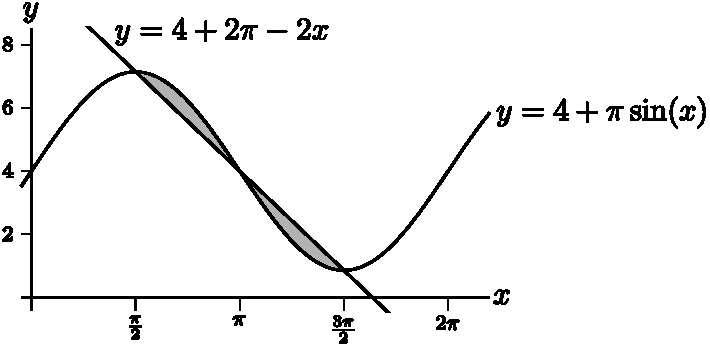
\includegraphics{OE13A_4a}
\end{center}

\noindent The region is rotated about the line $y = -1$.
Express in terms of definite integrals the volume of the resulting
solid. Do not evaluate the integrals.
\end{question}

\begin{hint}
Note that the curves cross. The area of this
region was found in Problem \ref{prob_s1.5q5} of Section 1.5.
It would be useful to review that problem.
\end{hint}

\begin{answer}
$\displaystyle\int_{\pi/2}^\pi \pi\big[(5 + \pi \sin x)^2-(5 + 2\pi - 2x)^2\big]\ \dee{x}
   +\displaystyle\int^{3\pi/2}_\pi \pi\big[(5 + 2\pi - 2x)^2-(5 + \pi \sin x)^2\big]\
            \dee{x}$
\end{answer}

\begin{solution}
We will compute the volume by rotating thin vertical strips as in
the sketch

\begin{center}
       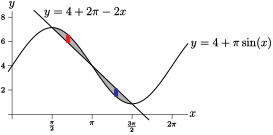
\includegraphics{OE13A_4}
\end{center}

\noindent
about the line $y=-1$ to generate thin washers.
We need to know when the line $y = 4 + 2\pi - 2x$ intersects the curve
$y = 4 + \pi \sin x$. Looking at the graph, it appears to be at $\frac{\pi}{2}$, $\pi$, and $\frac{3\pi}{2}$. By plugging in these values of $x$ to both functions, we see they are indeed the points of intersection.

\begin{itemize}
\item
When $\frac{\pi}{2} \le x \le \pi$, the top of the strip is at
$y = 4 + \pi \sin x$ and the bottom of the strip is at $y = 4 + 2\pi - 2x$.
When the strip is rotated, we get a thin washer with
outer radius $R_1(x)= 1+ 4 + \pi \sin x=5 + \pi \sin x $ and inner radius
$r_1(x) = 1+4 + 2\pi - 2x=5 + 2\pi - 2x$.
\item
When $\pi \le x \le \frac{3\pi}{2}$, the top of the strip is at
$y = 4 + 2\pi - 2x$ and the bottom of the strip is at $y = 4 + \pi \sin x$.
When the strip is rotated, we get a thin washer with outer radius
$R_2(x) = 1+4 + 2\pi - 2x=5 + 2\pi - 2x$ and inner radius
$r_2(x) = 1+ 4 + \pi \sin x=5 + \pi \sin x$.

\end{itemize}
So, the total
\begin{align*}
\hbox{Volume}
&= \int_{\pi/2}^\pi \pi\big[R_1(x)^2-r_1(x)^2\big]\ \dee{x}
   +\int^{3\pi/2}_\pi \pi\big[R_2(x)^2-r_2(x)^2\big]\ \dee{x}\\
&= \int_{\pi/2}^\pi \pi\big[(5 + \pi \sin x)^2-(5 + 2\pi - 2x)^2\big]\ \dee{x}
    \\ &\hskip0.5in
   +\int^{3\pi/2}_\pi \pi\big[(5 + 2\pi - 2x)^2-(5 + \pi \sin x)^2\big]\
            \dee{x}
\end{align*}
\end{solution}
%%%%%%%%%%%%%%%%%%%
\begin{Mquestion}\label{prob_s1.6:density}
%A rod with a circular cross section is one metre long, and has a constant diameter of
%10cm.
%It is manufactured so that, $x$ centimetres from one end, the density of the material is $ x~ \frac{\mathrm{g}}{{\mathrm{cm}^3}}$. What is the weight of the entire rod?

On a particular, highly homogeneous\footnote{This is clearly a simplified model: air density changes all the time, and depends on lots of complicated factors aside from altitude. However, the equation we're using is not so far off from an idealized model of the earth's atmosphere, taken from \emph{Pressure and the Gas Laws} by H.P. Schmid, \url{http://www.indiana.edu/~geog109/topics/10_Forces&Winds/GasPressWeb/PressGasLaws.html}, accessed 3 July 2017.} planet, we observe that the density of the atmosphere $h$ kilometres above the surface is given by the equation $\rho(h) = c2^{-h/6}\quad \frac{\mathrm{kg}}{\mathrm{m^3}}$, where $c$ is the density on the planet's surface.
\begin{enumerate}[(a)]
\item What is the mass of the atmosphere contained in a vertical column with radius one metre,  sixty kilometres high?
\item What height should a column be to contain $\dfrac{3000c\pi}{\log 2}$ kilograms of air?
\end{enumerate}
\end{Mquestion}
\begin{hint}
You can use ideas from this section to answer the question. If you take a very thin slice of the column, the density is almost constant, so you can find the mass. Then you can add up all your little slices. It's the same idea as volume, only applied to mass.

Do be careful about units: in the problem statement, some are given in metres, others in kilometres.

If you're having a hard time with the antiderivative, try writing the exponential function with base $e$. Remember $2 = e^{\log 2}$.
\end{hint}
\begin{answer}
(a) $\dfrac{6000c\pi}{\log 2}\left(1-\dfrac{1}{2^{10}}\right)$, which is close to
$\dfrac{6000c\pi}{\log 2}$.

(b) 6km: that is, there is roughly the same mass of air in the lowest 6 km of the column as there is in the remaining 54 km.
\end{answer}
\begin{solution}
(a)

We use the same ideas for volume, and apply them to mass. We want to take slices of the column, approximate their mass, then add them up. To reconcile our units, let $k=1000h$, so $k$ is the height in metres. Then the density of air at height $k$ is $c2^{-k/6000} ~\frac{\mathrm{kg}}{\mathrm{m}^3}$.

A horizontal slice of the column is a circular disk with height $\dee{k}$ and radius $1$ m. So, its volume is $\pi~ \dee{k}~\mathrm{m^3}$. What we're interested in, though, is its mass. At height $k$, its mass is
\begin{align*}
(\mathrm{volume})\times (\mathrm{density})&=\left(\pi ~\dee{k} ~\mathrm{m^3}\right)\times \left(c2^{-k/6000}~\frac{\mathrm{kg}}{\mathrm{m^3}}\right)\\
&=c\pi2^{-k/6000}~\dee{k}\quad\mathrm{kg}
\intertext{Since $k$ runs from 0 to $60,000$, the total mass is given by}
\int_0^{60000} c\pi2^{-k/6000}~\dee{k}&=c\pi\int_0^{60000} 2^{-k/6000}~\dee{k}
\intertext{To facilitate integration, we can write our exponential function in terms of $e$, then use the substitution $u=-\frac{k}{6000}\log 2$, $\dee{u} = -\frac{1}{6000}\log 2~\dee{k}$.}
&=c\pi\int_0^{60000}\left(e^{\log 2}\right)^{-k/6000}\dee{k}\\
&=c\pi\int_0^{60000}e^{-\tfrac{k}{6000}\log 2}\dee{k}\\
&=-\frac{6000c\pi}{\log 2}\int_0^{-10\log 2}e^{u}\dee{u}\\
&=\frac{6000c\pi}{\log 2}\int_{-10\log 2}^0e^{u}\dee{u}\\
&=\frac{6000c\pi}{\log 2}\left(1-\frac{1}{2^{10}}\right)
\end{align*}
We note this is fairly close to $\dfrac{6000c\pi}{\log 2}$.

We also remark that this is a demonstration of the usefulness of integrals. We wanted to know how much of \emph{something} there was, but the amount of that something was different everywhere: more in some places, less in others. Integration allowed us to account for this gradient. You've seen this behaviour exploited to find distances travelled, areas, volumes, and now mass. In your studies, you will doubtless learn to use it to find still more  quantities, and we will discuss other applications in Chapter~\eref{CLP101}{chap int app} of the CLP-2 text.

(b) We want to find the value of $k$ that gives a mass of $\dfrac{3000c\pi}{\log 2}$. By following our reasoning above, the mass of air in the column from the ground to height $k$ is
\begin{align*}
\frac{6000c\pi}{\log 2}\left(1-\frac{1}{2^{k/6000}}\right)&
\intertext{So, we set this equal to the mass we want, and solve for $k$.}
\frac{6000c\pi}{\log 2}\left(1-\frac{1}{2^{k/6000}}\right)&=\frac{3000c\pi}{\log 2}\\
2\left(1-\frac{1}{2^{k/6000}}\right)&=1\\
1&=\frac{2}{2^{k/6000}}\\
2^{k/6000}&=2^1\\
k&=6000\\
h&=6
\end{align*}

This means that there is roughly the same mass of air in the lowest 6 km of the column as there is in the remaining 54 km.
\end{solution}

%%%%%%%%%%%%%%%%%%%%
%
%\begin{question}
%A right circular cone with base radius $r$ and height $h$ is sliced vertically, as shown in the picture below. The cut is made so that the slice makes a chord across the circle sweeping out an angle of $\frac{\pi}{2}$ radians.
% Find the volume of the red piece.
%\begin{center}
%\hfill
%\begin{tikzpicture}
%\draw (0,0)node[shape=ellipse, minimum width=3cm, minimum height=1cm, draw] {};
%\draw (-1.5,0)--(0,3)--(1.5,0);
%\draw[dashed] (0,0)--(0,3) node[midway, left]{$h$};
%\draw[dashed] (0,0)--(-1.5,0) node[midway, below]{$r$};
%\draw[thick, fill=red, fill opacity=0.1] (-60:1.5cm and .5cm) arc (-60:60:1.5cm and .5cm) ;
%\filldraw[red, thick, left color=red!70!black, right color=white, fill, fill opacity=0.2] (.75,1.5)--(.75,-.4)arc (-60:0:1.5cm and .5cm) --cycle;
%\draw (0,-1) node{sliced cone};
%\end{tikzpicture}
%\hfill\begin{tikzpicture}
%\draw (0,0) node[shape=circle, minimum size=3cm, draw]{};
%\draw[dashed] (0,0)--(-1.5,0) node[below, midway]{$r$};
%\draw[red, fill=red, fill opacity=0.2] (0,0) + (45:1.5cm) arc (45:-45:1.5cm)--cycle;
%\draw (0,-2.) node{sliced base};
%\draw[dashed] (1.06,1.06)--(0,0)--(1.06,-1.06);
%\draw (.35,.35) arc(45:-45:.5cm) node[above right]{$\frac{\pi}{2}$};
%\end{tikzpicture}
%\hfill~
%\end{center}
%\end{question}
%\begin{hint}
%You'll want to use horizontal cross sections, like Example~\eref{CLP101}{eg:VOLa} of the
%CLP-2 text. Then the area of your slice can be calculated as a section of a circle, minus a triangle.
%\end{hint}
%\begin{answer}
%$ \dfrac{r^2h}{3}\left(\dfrac{\pi}{4}-\dfrac{1}{2}\right)$
%\end{answer}
%\begin{solution}
%As in Example~\eref{CLP101}{eg:VOLa} of the CLP-2 text, we take horizontal slices. If the radius of a slice is $s$, then its area can be calculated as one-quarter of the circle of radius $s$, minus the right triangle with base and height both $s$. So, \[A = \frac{1}{4}\left(\pi s^2\right) - \frac{1}{2} s^2 = s^2\left(\frac{\pi}{4}-\frac{1}{2}\right).\]
%
%As we climb up the cone, the radius of our slices changes. As in the text, let's assume that the base of the cone sits at $y=h$, and the tip is at $y=0$. Then we use similar triangles to conclude that at height $y$, the radius of the cone is $s=\left(\frac{r}{h}\right)y$.
%
%\begin{center}
%\begin{tikzpicture}
%\YEaaxis{1}{4}{1}{5}
%\YEycoord{2}{y}
%\YEycoord{4}{h}
%\YExcoord{3}{r}
%\draw (0,0)--(3,4)--(0,4);
%\fill[fill opacity=0.1] (0,0)--(1.5,2)--(0,2)--cycle;
%\draw (0,2)--(1.5,2);
%\draw (.75,2.25) node{$s$};
%\draw (5,3) node{$\dfrac{s}{y}=\dfrac{r}{h}$};
%\end{tikzpicture}
%\end{center}
%
%So:
%\begin{itemize}
%\item Our slices run from $y=0$ to $y=h$,
%\item at height $y$, the area of our slice is $\left(\frac{r}{h}\cdot y\right)^2\left(\frac{\pi}{4}-\frac{1}{2}\right) = y^2\left(\frac{r}{h}\right)^2\left(\frac{\pi}{4}-\frac{1}{2}\right)$,
%\item and the height of our slice is $\dee{y}$.
%\end{itemize}
%\item So, the volume of our piece of cone is:
%
%\begin{align*}
%\mbox{Volume}&=\int_0^h y^2\left(\frac{r}{h}\right)^2\left(\frac{\pi}{4}-\frac{1}{2}\right)\ \dee{y}\\
%&=\left(\frac{r}{h}\right)^2\left(\frac{\pi}{4}-\frac{1}{2}\right)\int_0^h y^2\ \dee{y}
%\\&=
%\left(\frac{r}{h}\right)^2\left(\frac{\pi}{4}-\frac{1}{2}\right)\frac{1}{3}h^3\\
%&= \frac{r^2h}{3}\left(\frac{\pi}{4}-\frac{1}{2}\right)
%\end{align*}
%\end{solution}


%%%%%%%%%%%%%%%%%%%%%%%%%%%%%%%%%%%%%
